\chapter{Results and Analysis}
\label{cha:results}

The primary objective of this study is to validate the efficacy of our Unpaired Image-to-Image Translation network, specifically CycleGAN, in bridging the domain gap between simulations and real-world orbital radar data, successfully discerning between noise and subsurface features via our anomaly detection pipeline.
This chapter details the experimental methodology, analyzes the generative performance of the proposed models, and evaluates the downstream utility of the synthetic data for anomaly detection tasks.
We begin by outlining the experimental setup, including dataset curation, hardware specifications, and the quantitative metrics employed for evaluation.

\section{Experimental Setup}
\label{sec:experimental_setup}
To ensure the reproducibility and scientific validity of our results, a rigorous experimental framework was established.
The core of our investigation relies on a custom PyTorch implementation designed to handle the unique constraints of SHAllow RADar (SHARAD) data, with a standardized hyperparameter configuration optimized for the specific characteristics of the dataset and the network architectures.
The following subsections describe the data acquisition process and the multi-faceted metric suite used to quantify generative realism.
The hyperparameter configurations used during the training campaigns, including learning rates, optimization strategies, and loss weighting, were previously established and are summarized in Table~\ref{tab:hyperparams} (Section~\ref{sec:modular_implementation}).
For a complete list of the configuration states and environment variables used across all runs, the reader is referred to Appendix~\ref{app:reproducibility}.

\subsection{Selection of Regions of Interest (ROIs)}
\label{subsec:roi_selection}
The selection of the training and testing datasets for this study was driven by a strategic geological assessment rather than random sampling.
The efficacy of a generative model in scientific applications is contingent upon the quality and representativeness of the input data.
Consequently, we identified two distinct Martian regions to serve disjoint roles in the training and validation pipeline: the Elysium Planitia for learning the background distribution, and a specific targeted strip for validating the anomaly detection capabilities.

\subsubsection{Training Set: Elysium Planitia and The \enquote{Big Data} Approach}
For the construction of the training set, a \enquote{quantity-first} approach was adopted.
Deep generative models, particularly those based on the GAN framework, are notoriously data-hungry, requiring vast amounts of varied examples to learn robust internal representations and avoid mode collapse.
To satisfy this requirement, we selected the entire \textbf{Elysium Planitia} region as our primary source of training data.

From a geological perspective, Elysium Planitia is characterized as a vast volcanic region dominated by extensive lava plains.
The surface exhibits notably \textbf{low topographic roughness}, minimizing the complexity of off-nadir surface clutter that often complicates radar interpretation.
Ideally suited for this task, the subsurface stratigraphy consists of \textbf{regular subsurface layering} resulting from sequential episodes of lava flows.
This geometric regularity is crucial for the stability of the Generative Adversarial Network.

This choice resulted in a large dataset consisting of approximately \textbf{1600 raw radar observation pairs}.
By ingesting the entire zone, we effectively capture the full variance of the Martian subsurface in this region, including a wide spectrum of noise profiles, surface clutter types, and geological features.

It is important to acknowledge the trade-off inherent in this strategy.
By including the comprehensive set of observations from Elysium Planitia without granular manual filtering, the training set inevitably contains a percentage of \enquote{noisy} or \enquote{less useful} samples, represented by radargrams where the signal might be too attenuated, the subsurface features distinctively absent, or the thermal noise dominant.
However, recent literature in deep learning suggests that large-scale neural networks are remarkably robust to label noise and can benefit from the regularization effect provided by a diverse, though imperfect, dataset.

The consistent, parallel nature of the stratigraphic sequences allows the neural network to learn the "texture" of the SHARAD instrument's noise response and the dielectric behavior of the surface without being confounded by chaotic scattering or complex tectonic deformation.
The network is forced to learn the \enquote{common denominator}, specifically the underlying physics of radar reflection and the general structure of subsurface layers, rather than overfitting to a small, manually curated subset.
It serves as the "control" dataset, enabling the model to internalize the rules of radar signal propagation in a standard Martian regolith.

\subsubsection{Test Set: Precision, Human Validation \& Anomaly Verification}
In contrast to the training set, the validation of the anomaly detector requires a target that deviates from the learned norm.
We designated a specific Region of Interest (ROI) bounded by coordinates [172$^{\circ}$E--174$^{\circ}$E, 7$^{\circ}$N--8$^{\circ}$N].

This area was selected based on a preliminary visual inspection of SHARAD radargrams, which revealed the presence of \textbf{marked subsurface reflectors}.
These strong dielectric contrasts are potentially indicative of buried massive ice deposits or distinct interfaces between differing geological materials.

To ensure the highest quality for evaluation, the test set was constructed through a rigorous, manual selection process.
Therefore, the large-scale ingestion strategy adopted during training was not considered suitable for the construction of the test set.
For the test set, several hundred radargrams were visually examined to identify specific \enquote{Golden Samples}, defined as regions satisfying the following criteria:

\begin{itemize}
    \item Clearly discernible and unambiguous subsurface layering.
    \item Favorable signal-to-noise ratio (SNR), enabling reliable comparison between reconstructed and original data.
    \item Geological features representative of the principal structures under investigation (e.g., well-defined interfaces or potential anomalies).
\end{itemize}

This human-in-the-loop selection procedure ensures that both quantitative metrics (e.g., SSIM, PSNR) and qualitative evaluations are grounded in scientifically meaningful examples.
It further prevents the evaluation results from being biased by low-quality input data, for which even an ideal reconstruction would remain indistinguishable from noise.

The rationale for this selection is to test the \textbf{generalization capability} of the anomaly detector by presenting it with an "exception" to the rules learned from Elysium.
Since the electromagnetic simulator used to generate the input paired data does not account for these specific subsurface structures (being based solely on surface topography), the CycleGAN—trained to reproduce the simulation's logic—is expected to generate a "blind" reconstruction that lacks these features.
Consequently, a comparison between the generated "background-only" image and the real radargram (containing the reflectors) should yield a high-intensity difference map specifically at these coordinates.
This discrepancy serves as our "Ground Truth" for validating the sensitivity and accuracy of the anomaly detection algorithm, distinguishing its true performance from its ability to merely reproduce background noise.

\subsection{Dataset Composition \& Preprocessing}
\label{subsec:dataset}
The dataset employed in this study is derived from the SHallow RADar (SHARAD) instrument onboard the Mars Reconnaissance Orbiter (MRO), specifically targeting the Elysium Planitia region.
The complete dataset comprises approximately 1,600 unique radargrams, which were rigorously curated to ensure a representative distribution of Martian subsurface features.
To facilitate a robust learning process and monitor generalization capability, the dataset was partitioned following a standard split: 80\% of the data ($N \approx 1280$) was allocated for training, while the remaining 20\% ($N \approx 320$) constituted the validation set used for hyperparameter tuning and early stopping. Additionally, a distinct set of radargrams ($N = 10$, which resulted in 60 patches) was strictly reserved for the final testing phase to evaluate the model on unseen geographies.

The raw data requires a specialized pre-processing pipeline, implemented within the project's \texttt{MapDataset} module, to be suitable for deep learning applications.
Initially, the raw radar echoes are loaded using the \texttt{pdr} library and converted into a logarithmic decibel scale to compress the high dynamic range of the signal. Subsequently, a global Min-Max normalization is applied, rescaling the pixel intensity values to the range $[-1, 1]$.
This normalization step is critical for stabilizing the training of the Generative Adversarial Network, matching the output range of the generator's Tanh activation function.
Finally, instead of processing entire radargrams, which can exceed $3600 \times 1000$ pixels, the images are tessellated into square patches of $128 \times 128$ pixels.
This patching strategy serves a dual purpose: it drastically reduces peak Video RAM (VRAM) requirements, allowing for efficient training on standard GPU hardware, and it increases the effective size of the dataset, providing the model with a diverse set of local textural examples independent of global stratigraphy.

\subsection{Hardware \& Implementation Details}
\label{subsec:hardware}
As detailed in Chapter~\ref{cha:methodology}, the experimental pipeline relies on a modular, containerized PyTorch architecture.
While initial prototyping occurred locally, the extensive training campaigns presented in this chapter were executed on a Linux-based High-Performance Computing (HPC) cluster equipped with NVIDIA GPUs. 

The Docker-based setup ensured perfect reproducibility across these environments without procedural overhead.
During the training phase, Automatic Mixed Precision (AMP) and custom CUDA-accelerated routines were heavily utilized to maximize throughput and minimize the VRAM footprint.
Finally, the systematic exploration of the hyperparameter space was orchestrated by the Optuna framework, which was seamlessly integrated into the training loops to empirically determine the optimal configuration for the generative models.

\subsection{Evaluation Metrics}
\label{subsec:evaluation_metrics}
Quantifying the performance of generative models in unpaired image-to-image translation requires a composite evaluation protocol that assesses both pixel-level fidelity and perceptual realism.
As previously introduced and theoretically defined in Section~\ref{sec:anomaly_detection_methodology}, we employ a specific suite of metrics, namely Peak Signal-to-Noise Ratio (PSNR), Structural Similarity Index (SSIM), and Learned Perceptual Image Patch Similarity (LPIPS), to evaluate the model outputs.
Rather than redefining their mathematical formulation, this section outlines how they are applied in practice to score the generative fidelity of the translated radargrams:

\begin{itemize}
    \item \textbf{Peak Signal-to-Noise Ratio (PSNR):} Derived directly from the Mean Squared Error (MSE), PSNR is used to measure the baseline pixel-wise reconstruction error. While a high PSNR implies low numerical deviation, in the context of radar sounding it correlates poorly with human perception of \enquote{realism}. We track it primarily as a sanity check for model convergence, noting its extreme sensitivity to the small spatial misalignments common in unpaired translation.
    \item \textbf{Structural Similarity Index (SSIM)~\cite{Wang_2004}:} In our operational pipeline, SSIM evaluates the preservation of structural geology. Since the continuity and relative geometry of subsurface horizons carry most of the scientific information (rather than absolute pixel intensities), SSIM serves to penalize models that distort or hallucinate stratigraphy during the translation process.
    \item \textbf{Learned Perceptual Image Patch Similarity (LPIPS)~\cite{Zhang_2018_CVPR}:} This metric is utilized to assess how closely the synthesized radargrams match the perceptual texture and stochastic speckle statistics of real SHARAD data. Being robust to the minor spatial shifts that heavily penalize PSNR, LPIPS acts as our primary proxy for evaluating the true generative realism of the CycleGAN.
\end{itemize}

These metrics are automatically computed by the \texttt{compare\_models.py} framework and reported both as dataset-wide averages and as full probability distributions, allowing us to capture the variance of generative quality across different Martian topographies.



\section{Comparative Generative Quality}
\label{sec:comparative_generative_quality}

To systematically present our findings and provide a clear roadmap of the experiments, this chapter follows a structured progression:
\begin{itemize}
    \item \textbf{Model Selection (Section~\ref{subsec:model_selection}):} We evaluate paired (Pix2Pix) versus unpaired (CycleGAN) translation frameworks to identify the optimal architecture for Martian radar data.
    \item \textbf{Results of the GAN Comparison (Section~\ref{subsec:gan_comparison_results}):} We quantitatively and qualitatively benchmark the competing models using structural and perceptual metrics.
    \item \textbf{Sensitivity Analysis (Section~\ref{sec:sensitivity_analysis}):} We explore the impact of specific hyperparameters (e.g., patch size and loss weighting) on the generative quality.
    \item \textbf{Anomaly Detection Application (Section~\ref{sec:anomaly_detection_application}):} We deploy the optimal generator to isolate and detect subsurface anomalies.
\end{itemize}

\subsection{Model Selection Strategy}
\label{subsec:model_selection}

We began our experimental phase by selecting an appropriate generative architecture based on the relationship between the physical simulations and the observational data.
We initially evaluated Pix2Pix (previously detailed in Section~\ref{sec:modular_implementation}), a conditional GAN framework requiring paired image samples. 

We based this choice on the assumption that our physical approximations aligned spatially with the real radargrams.
We anticipated that the strong pixel-level supervision from the $L1$ regression loss would force the generator to directly superimpose realistic noise onto the simulations. 

However, empirical results revealed fundamental spatial misalignments, invalidating the paired assumption.
The Pix2Pix model rapidly overfit and generated high-frequency artifacts.
Instead of learning the SHARAD instrument's noise distribution, the network memorized specific training pairs.
The resulting images exhibited either excessive blurring (as the model averaged outcomes to minimize $L1$ error) or distinct checkerboard artifacts, failing to reproduce the stochastic clutter.

Consequently, we pivoted to the unpaired CycleGAN framework.
Simulated and real data share valid semantic content (subsurface stratigraphy) but lack strict pixel-to-pixel correspondence due to orbital positioning errors and simplified simulation physics. 

CycleGAN addresses this misalignment through the Cycle Consistency Loss, which enforces transitivity.
By requiring the round-trip translation ($A \rightarrow B \rightarrow A \approx A$) to match the original input, the model preserves structural information.
This mechanism allows the generator to adapt the surface clutter and add speckle noise without destroying the primary geological reflectors.
Only the genuine structural features survive the round-trip translation.

We highlight a critical trade-off: the balance between pixel-level accuracy and domain consistency.
Pix2Pix optimizes for numerical proximity rather than perceptual realism, making it unstable when processing imperfectly aligned scientific data.
CycleGAN relaxes the spatial constraint and prioritizes the statistical alignment of feature distributions.
We demonstrated that this domain-consistent approach is significantly more robust for SHARAD data.
CycleGAN generated sharper, more realistic textures and maintained the integrity of subsurface horizons.
These outputs proved highly suitable for downstream anomaly detection algorithms relying on structural coherence.


\subsection{Results of the GAN Comparison}
\label{subsec:gan_comparison_results}

We quantitatively and qualitatively compare the CycleGAN architecture with the Pix2Pix baseline.
We trained both models on the same dataset split and evaluated them on the test set using the metrics defined in Section~\ref{subsec:evaluation_metrics}.
We aim to understand how different training objectives affect the perceptual realism of the generated radargrams and their suitability for downstream anomaly detection.

\subsubsection{Quantitative and Qualitative Benchmarking}
Table~\ref{tab:benchmark_pix2pix_cyclegan} reports the average PSNR, SSIM, and LPIPS scores for both models.
Classical pixel-wise metrics (PSNR and SSIM) show similar results for Pix2Pix and CycleGAN, suggesting both networks reproduce the global structure of the radargrams at a coarse level.
We observe $PSNR_{\text{cyc}} \approx 23.0$~dB versus $PSNR_{\text{pix}} \approx 19.0$~dB, and comparable SSIM values.
Both models reconstruct large-scale stratigraphic interfaces and surface echoes with similar mean squared error and structural similarity.

\begin{table}[htbp]
    \centering
    \caption{Quantitative comparison between Pix2Pix and CycleGAN on the test set. The values are obtained from the benchmark script and correspond to mean scores over all test samples.}
    \label{tab:benchmark_pix2pix_cyclegan}
    \begin{tabular}{lcccc}
        \hline
        Model    & PSNR [dB] $\uparrow$ & SSIM $\uparrow$ & LPIPS $\downarrow$ & FID $\downarrow$ \\
        \hline
        Pix2Pix  & 19.0      & 0.234 & 0.254 & 11.03 \\
        CycleGAN & \textbf{23.0}      & \textbf{0.291} & \textbf{0.104} & \textbf{1.56} \\
        \hline
    \end{tabular}
\end{table}

However, the Learned Perceptual Image Patch Similarity (LPIPS) metric, introduced by Zhang et al.~\cite{Zhang_2018_CVPR}, reveals a pronounced difference.
The CycleGAN model attains a significantly lower LPIPS score ($0.104$) compared to Pix2Pix ($0.254$).
In the feature space of a deep convolutional network, CycleGAN outputs are perceptually closer to real SHARAD observations.
Figure~\ref{fig:lpips_distribution} illustrates these empirical distributions.

\begin{figure}[htbp]
    \centering
    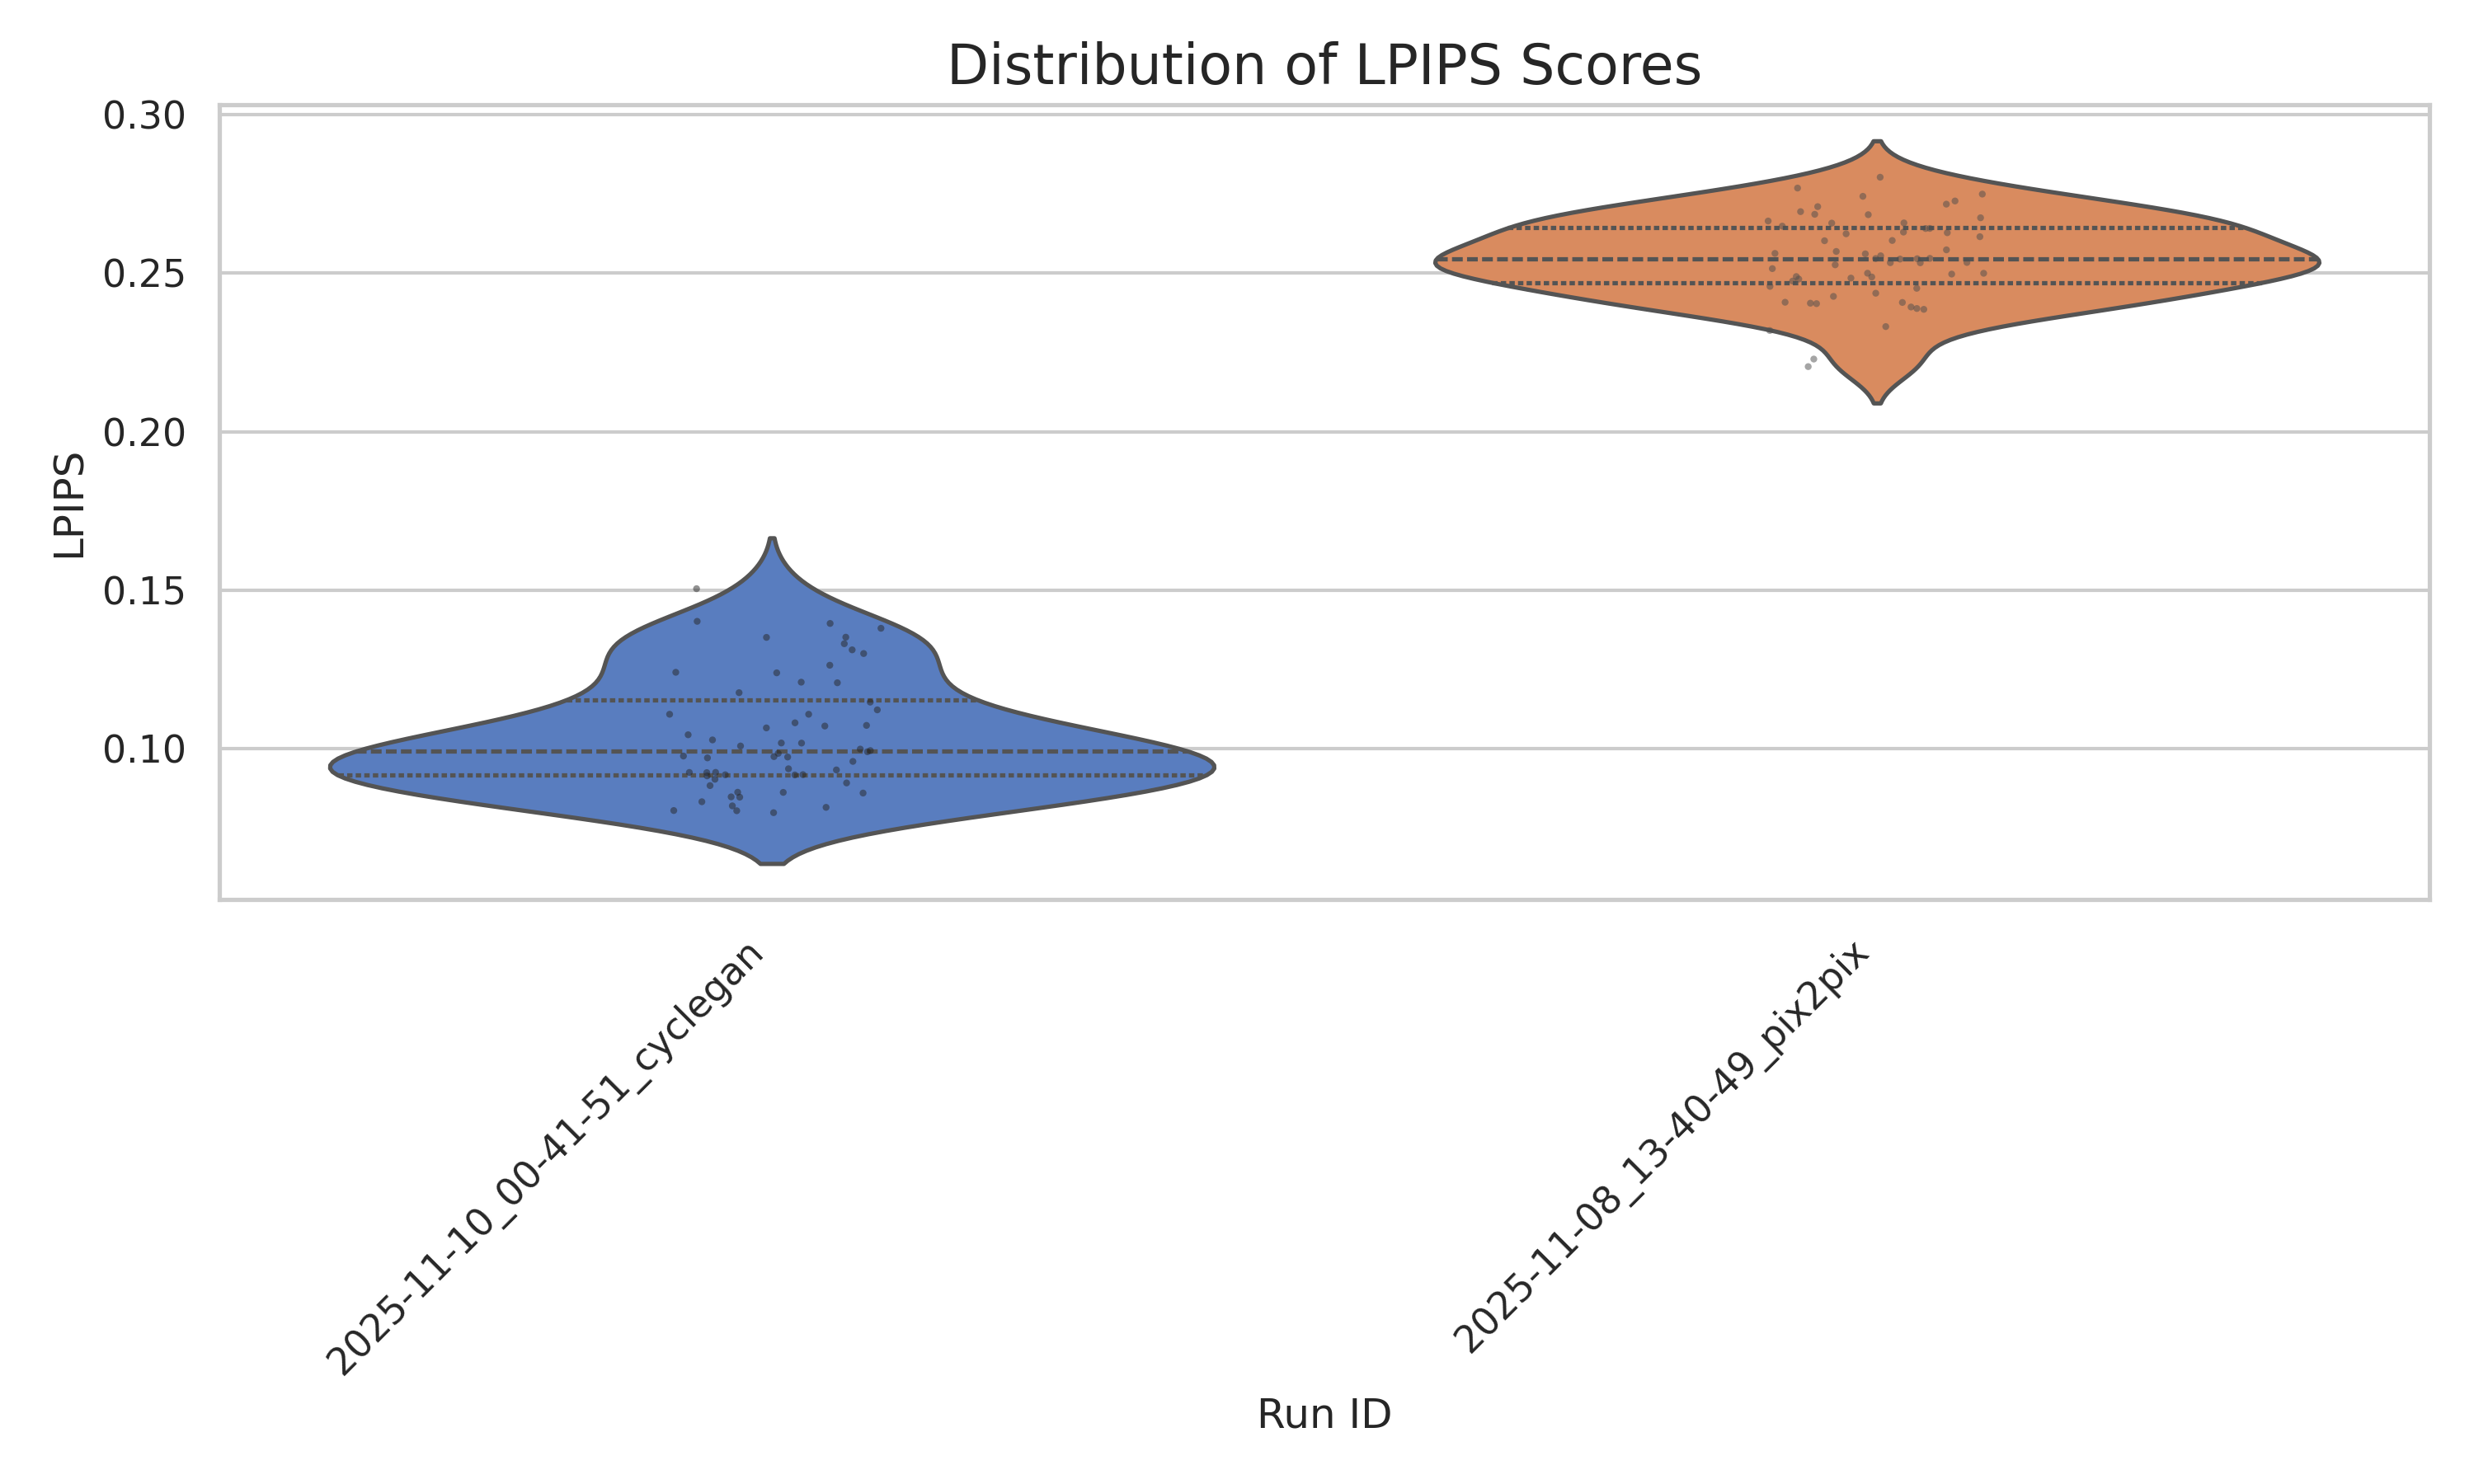
\includegraphics[width=0.6\textwidth]{images/benchmark/lpips_distribution.png}
    \caption{Distribution of the Learned Perceptual Image Patch Similarity (LPIPS) scores evaluated on the test set. The CycleGAN model exhibits a tightly clustered distribution with a significantly lower mean distance (0.104) compared to the wider, high-variance distribution of the Pix2Pix baseline (0.254). Lower values indicate generated textures that are perceptually closer to real Martian radargrams.}
    \label{fig:lpips_distribution}
\end{figure}

We confirm this interpretation through qualitative visual comparisons (see Figure~\ref{fig:qualitative_comparison}).
Driven by a strong L1 regression loss, Pix2Pix minimizes the average error by blending multiple plausible outcomes.
This mechanism causes excessive blurring and a loss of fine-scale texture.
The model blurs thin subsurface horizons and strongly attenuates the speckle pattern.
It yields images that are numerically close to the target but lack the characteristic \enquote{grain} of real radar data.

In contrast, CycleGAN leverages its adversarial loss and PatchGAN discriminator to match the local texture statistics of the real domain.
The objective function explicitly encourages the generator to synthesize realistic high-frequency speckle noise and small-scale clutter, tolerating minor pixel-level misalignments.
Consequently, the reconstructed radargrams preserve the \enquote{crispness} of the SHARAD signal. Hyperbolic diffractions, background noise, and subtle layering exhibit a granular appearance visually similar to real acquisitions.
This behavior directly benefits the subsequent anomaly detection pipeline.
It prevents artificial smoothness, which would otherwise generate spurious residuals and false positives when comparing real radargrams against synthetic baselines.

\begin{figure}[htbp]
    \centering
    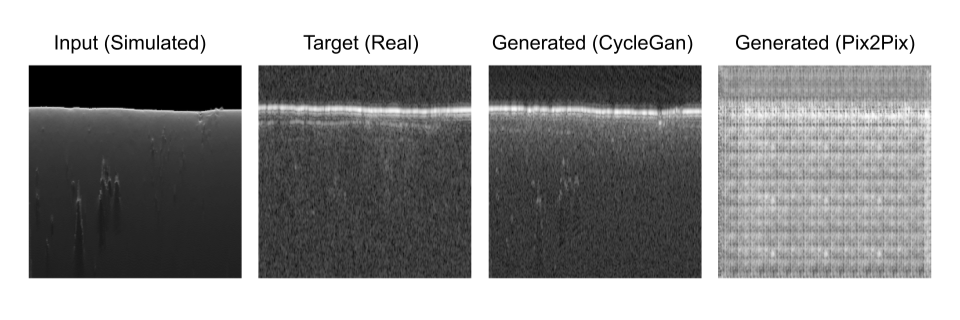
\includegraphics[width=\textwidth]{images/benchmark/comparison_sample_4}
    \caption{Qualitative comparison of Sim-to-Real translations. While the paired Pix2Pix model tends to average out structural details, leading to severe blurring artifacts and a loss of physical realism, the unpaired CycleGAN architecture preserves coherent stratigraphic horizons and synthesizes realistic high-frequency speckle noise characteristic of the real SHARAD domain. This visual behaviour is consistent with the significant gap in LPIPS and FID scores reported in Table~\ref{tab:benchmark_pix2pix_cyclegan}.}
    \label{fig:qualitative_comparison}
\end{figure}

\subsubsection{Feature Distribution Analysis}
To assess the generative consistency across diverse geological scenarios, we analyze the full probability density function of the scores rather than relying solely on dataset-wide averages.
As shown in Figure~\ref{fig:lpips_distribution}, we utilize \textbf{Violin Plots} to visualize these distributions.
The CycleGAN model exhibits a tightly clustered LPIPS distribution, indicating that it consistently produces high-quality textures across all tested patches.
In contrast, the Pix2Pix baseline shows a wider, high-variance distribution.
This visualization confirms that CycleGAN improves not just the average \textit{quality} of the generation, but also its \textit{reliability}, a critical requirement for scientific applications.

\subsubsection{Inference Efficiency and Reproducibility}
Beyond perceptual quality, we profiled the computational cost of the selected architectures.
We logged the inference time per patch during the benchmark loop to assess feasibility for planetary-scale processing.
For the deployed CycleGAN architecture ($128 \times 128$ patch input), the model achieves a mean inference latency of $\approx 4.2$~ms on an NVIDIA RTX 3090.
This performance confirms the system's viability for the real-time processing of massive orbital data streams.

Finally, to guarantee scientific rigor, the evaluation framework systematically versions all artifacts.
The system exports raw CSV metrics, high-resolution comparison grids, and summary JSON reports into timestamped output directories.
This ensures we can trace every experimental claim back to a specific, reproducible software execution context.


\section{Sensitivity Analysis}
\label{sec:sensitivity_analysis}
We refined the CycleGAN performance by tuning two critical hyperparameters: input patch size and cycle-consistency loss weight.

\subsection{Impact of Patch Size}
The input patch size defines the generator's receptive field.
We evaluated four resolutions: $64 \times 64$, $128 \times 128$, $256 \times 256$, and $512 \times 512$ pixels (see visual comparisons in Figure~\ref{fig:patch_size_comparison}).

\begin{figure}[htbp]
    \centering
    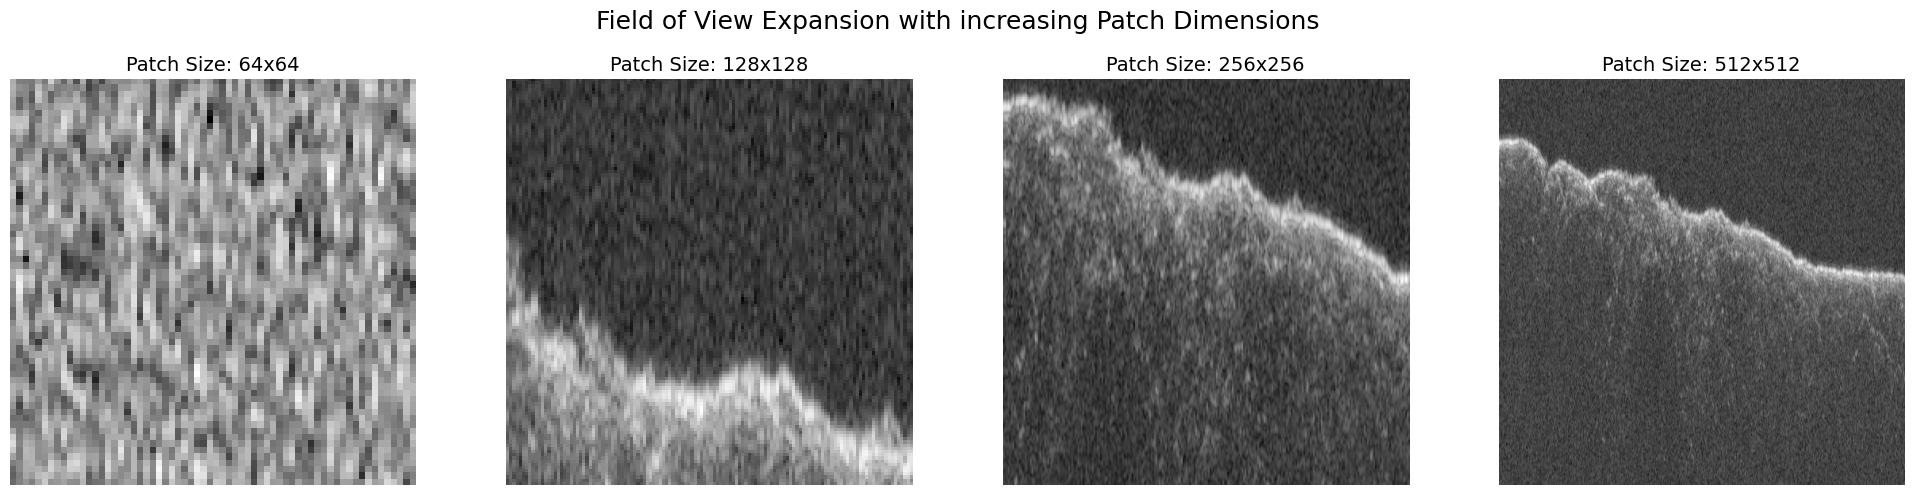
\includegraphics[width=\textwidth]{images/example_plots/ID_01970402/varying_patch_sizes}
    \caption{Field of View expansion with increasing patch dimensions. From left to right: $64\times64$, $128\times128$, $256\times256$, and $512\times512$ pixels, all extracted from the same radargram location. At $64\times64$, the receptive field is too narrow to resolve any coherent stratigraphic structure, yielding a texture-only view devoid of geological context. At $128\times128$, the principal surface echo and the transition into the subsurface noise floor are both visible, providing sufficient context for training. Larger patches ($256\times256$ and $512\times512$) progressively include the deep, signal-poor region of the radargram, diluting the informative content and increasing memory overhead without a corresponding gain in structural detail.}
    \label{fig:patch_size_comparison}
\end{figure}

Small patches ($64 \times 64$) restrict the effective spatial context, or Field of View (FoV).
The model fails to capture the continuity of long subsurface reflectors, causing layers to abruptly end at patch boundaries.

Conversely, $512 \times 512$ patches consume excessive VRAM, forcing a batch size of 1.
This causes noisy gradients and unstable training.
Moreover, large patches include deep, signal-poor regions that provide no useful features.

We identified $128 \times 128$ as the optimal size.
It captures essential geological structures (horizontal layers and hyperbolic diffractions) while maintaining a stable batch size.
Physically, 128 pixels cover $\approx 2$ km of depth, providing enough context for shallow anomalies without wasting computation.

\subsection{Weighting the Cycle-Consistency Loss}
The parameter $\lambda_{cycle}$ controls the contribution of the cycle-consistency loss relative to the adversarial loss.
It dictates the penalty for altering the image's structural content:

$$L_{total}=L_{GAN}+\lambda_{cycle}L_{cyc}$$

Through empirical validation on the validation set, we determined that $\lambda_{cycle}=10.0$ provides the optimal balance. 

A low $\lambda_{cycle}$ gives the generator excessive freedom.
While the model generates plausible radar textures, it geometrically distorts or entirely fabricates subsurface layers, destroying the physical validity of the synthetic data.

Conversely, an excessively high $\lambda_{cycle}$ constrains the generator to perform an identity mapping.
The model perfectly preserves the geometry but fails to inject the requisite speckle noise and thermal clutter, defeating the purpose of domain adaptation.

A weighting of 10.0 is strong enough to enforce the strict preservation of the principal stratigraphic horizons.
Simultaneously, it allows the adversarial network to successfully overlay the high-frequency noise texture characteristic of the SHARAD sensor.


\section{Anomaly Detection Application}
\label{sec:anomaly_detection_application}

Having validated the CycleGAN architecture and selected the optimal cycle-consistency weight, we now apply the model to detect subsurface anomalies.
We define an anomaly as a dielectric discontinuity present in the real data but absent in the surface-only simulation (e.g., ice deposits or deep stratigraphy).

\subsection{Residual-Based Detection Pipeline}
\label{subsec:residual_pipeline}

The proposed anomaly detection framework relies on a \textbf{residuals-based approach}.
We leverage the learned translation mapping $G_{Sim \to Real}$ to construct a coherent \enquote{reference background} for every acquired radargram.
The procedure assumes that the simulation domain represents a \enquote{clutter-only} control scenario, effectively isolating surface reflections calculated via geometric optics.

The detection pipeline consists of three sequential stages:
\begin{enumerate}
    \item \textbf{Synthetic Domain Adaptation:} We project the deterministic simulation $x_{sim}$ into the realistic RS domain using the generator. The output, $x_{gen} = G_{Sim \to Real}(x_{sim})$, retains the structural topology of the surface reflections but lacks subsurface features, perfectly mimicking the background noise and clutter.
    \item \textbf{Difference Amplification:} We compute the absolute element-wise difference between the empirical observation $x_{real}$ and the synthetic reference $x_{gen}$. This yields the Residual Map $\mathcal{M} = |x_{real} - x_{gen}|$. The subtraction cancels out the strong surface returns (clutter), leaving only the energy of genuine subsurface anomalies.
    \item \textbf{Thresholding and Segmentation:} We apply a discrimination threshold $\tau$ to convert the continuous energy values of $\mathcal{M}$ into a binary detection map $M$, highlighting candidate Regions of Interest (ROI) where the dielectric response significantly deviates from the surface-only prediction.
\end{enumerate}

Among the difference metrics evaluated (L1, SSIM, LPIPS) and the aggregation strategies considered (pixel-level, patch-based, sliding-window), the combination of the L1 metric with sliding-window averaging provided the most balanced trade-off between spatial detail, noise robustness, and anomaly coherence.
This configuration was therefore adopted as the standard pipeline for all subsequent experiments.

\subsection{Qualitative Analysis of Injected Dipping Layers and Failure Modes}
\label{subsec:qualitative_injected_layers}

Beyond aggregate ROC and PR metrics, a qualitative inspection of individual detections is essential to understand \emph{how} the model succeeds and \emph{where} it fails.
The residual maps obtained from the Synthetic Anomaly Injection experiments (e.g., Figure~\ref{fig:synthetic_anomaly_example}) confirm the intended behavior of the generator $G_{Sim \to Real}$: it reliably reconstructs the background distribution characteristic of the Elysium Planitia training region—dominated by quasi-parallel subsurface layers and moderate speckle—while being unable to reproduce out-of-distribution structures such as the injected dipping layers.
Since the latter have no counterpart in the input simulation domain, the generator tends to \enquote{hallucinate} a clean, layer-like background in their place.
The subsequent subtraction $|y_{\text{real, injected}} - \hat{y}_{\text{clean}}|$ therefore isolates the anomaly as a coherent residual, as desired.
Simultaneously, the generator preserves the background clutter structure, so that only genuinely out-of-distribution energy contributes to elevated residual values.

At the same time, qualitative analysis also reveals systematic failure modes.
In regions of extremely high surface roughness or complex topography, the geometric-optics-based simulation may diverge substantially from the real radargram, causing the CycleGAN to produce residual maps with localized high-energy regions that are indistinguishable from true anomalies, thereby generating false positives.
A representative example is shown in Figure~\ref{fig:failure_mode_example}.

\begin{figure}[htbp]
    \centering
    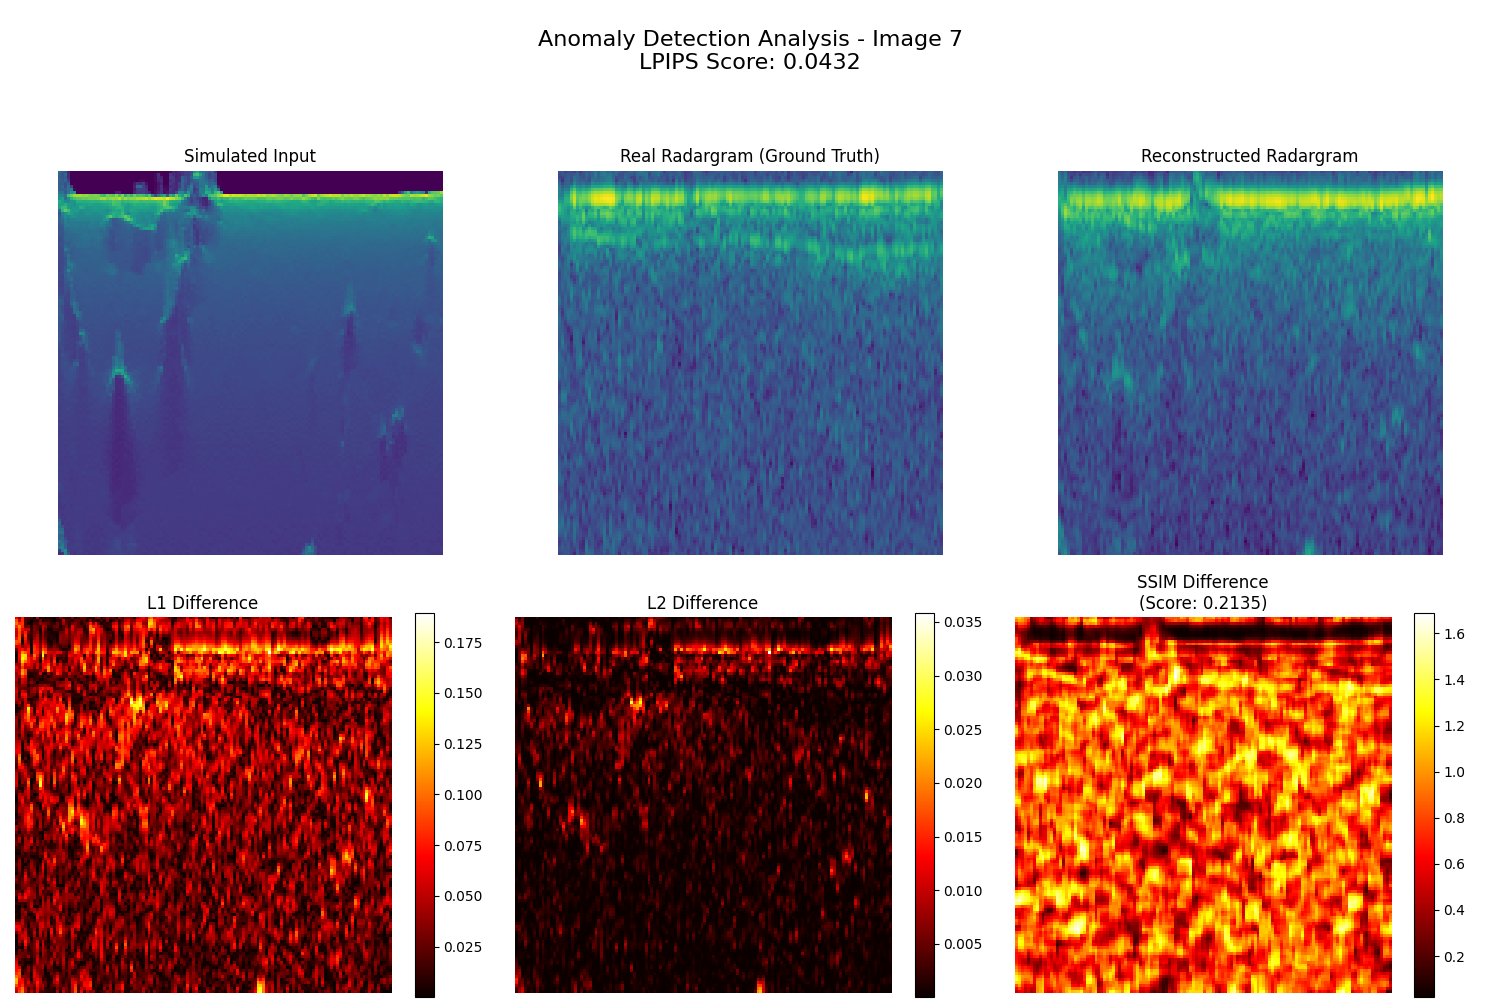
\includegraphics[width=\textwidth]{images/2025-12-26_15-13-28_experiment_run_ALL/00_baseline_raw/0007_matplotlib_comparison}
    \caption{Representative reconstruction example illustrating a failure mode in regions of strong surface clutter. Top row: (a) simulated radargram used as input to the CycleGAN, (b) corresponding real radargram (ground truth), and (c) reconstructed radargram generated by $G_{Sim \to Real}$. Bottom row: residual maps highlighting discrepancies between the reconstruction and the real observation, shown as (d) $L_1$ difference, (e) $L_2$ difference, and (f) SSIM-based structural difference. The structured high-energy regions in the residual maps arise from complex surface scattering that is not captured by the geometric-optics-based simulator, leading the anomaly detector to produce false positives in high-roughness areas.}
    \label{fig:failure_mode_example}
\end{figure}


A complementary failure mode arises when $G_{Sim \to Real}$ is overly aggressive in suppressing clutter, attenuating not only surface-related hyperbolas but also portions of genuine subsurface reflectors.
When such partial attenuation overlaps with the injected layer, the residual map becomes ambiguous: the anomaly signal is diluted by reconstruction errors, highlighting the fundamental trade-off between clutter suppression and anomaly preservation.

Overall, this qualitative analysis provides a more complete picture of the detector's behavior.
On the one hand, the residual-based strategy effectively amplifies out-of-distribution subsurface features when the simulation and real data are reasonably aligned.
On the other hand, it remains sensitive to domain mismatches induced by extreme surface roughness or limitations of the forward simulator, which manifest as structured false positives in the residual maps.
These observations motivate the physics-informed and adaptive-thresholding extensions discussed in Chapter~\ref{cha:conclusion}.

\subsection{Quantitative Evaluation on Synthetic Injections}
\label{subsec:quantitative_anomaly_detection}
To quantitatively assess the pipeline, we evaluated the model using the Synthetic Anomaly Injection protocol defined in Section~\ref{sec:synthetic_anomaly_injection}.
Each real radargram in the test subset is augmented with a synthetic dipping layer.
This generates controlled, physically plausible anomalies with known ground truth masks.
We applied the detection pipeline to these augmented samples to produce pixel-level anomaly scores.

Figure~\ref{fig:roc_pr_curves} shows the Receiver Operating Characteristic (ROC) and Precision–Recall (PR) curves obtained by thresholding the residual scores against the ground truth masks.

\begin{figure}[htbp]
    \centering
    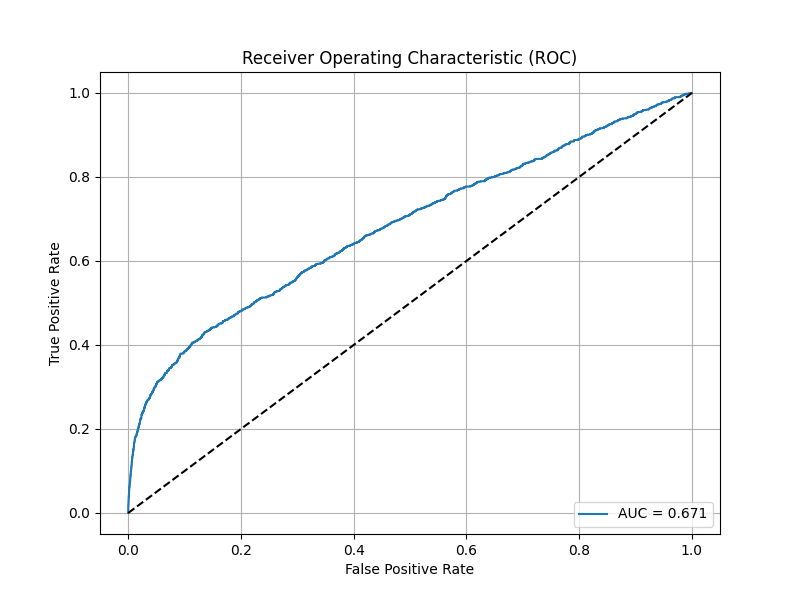
\includegraphics[width=0.48\textwidth]{images/anomaly_eval/roc_curve.png}
    \hfill
    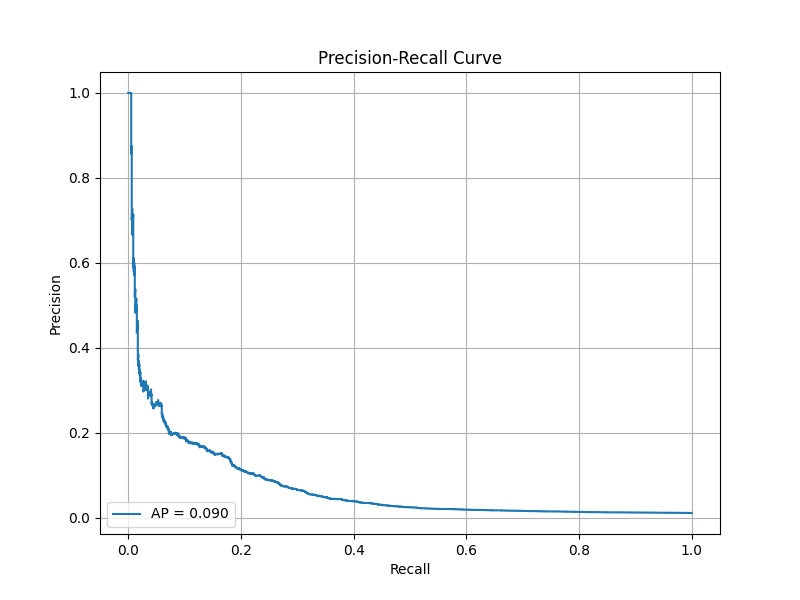
\includegraphics[width=0.48\textwidth]{images/anomaly_eval/pr_curve.png}
    \caption{Quantitative evaluation of the anomaly detector on synthetic dipping-layer injections. Left: Receiver Operating Characteristic (ROC) curve with an AUC of $0.671$. Right: Precision-Recall (PR) curve with a Mean Average Precision (mAP) of $0.089$.}
    \label{fig:roc_pr_curves}
\end{figure}

The system attains an Area Under the ROC Curve (AUC) of $0.671$.
This indicates a robust discriminative capability, substantially above the random-guess baseline of $0.5$.
Pixels belonging to the injected dipping layers systematically exhibit higher residual values than background pixels.
This confirms that the learned Sim-to-Real translation effectively normalizes clutter and highlights novel subsurface reflectors.

The Precision–Recall analysis yields a Mean Average Precision (mAP) of $0.089$.
As expected in a highly imbalanced and noise-dominated scenario, precision decreases at very high recall levels.
Aggressive thresholds recover almost all anomalous pixels but also admit false positives due to residual speckle fluctuations.
However, within a practical operating regime, the detector successfully flags significant subsurface features while keeping the false alarm rate acceptable.

Figure~\ref{fig:synthetic_anomaly_example} illustrates the behavior at the sample level.
The residual image clearly highlights the injected feature as a coherent, high-intensity structure, despite the presence of strong background clutter and speckle.

\begin{figure}[htbp]
    \centering
    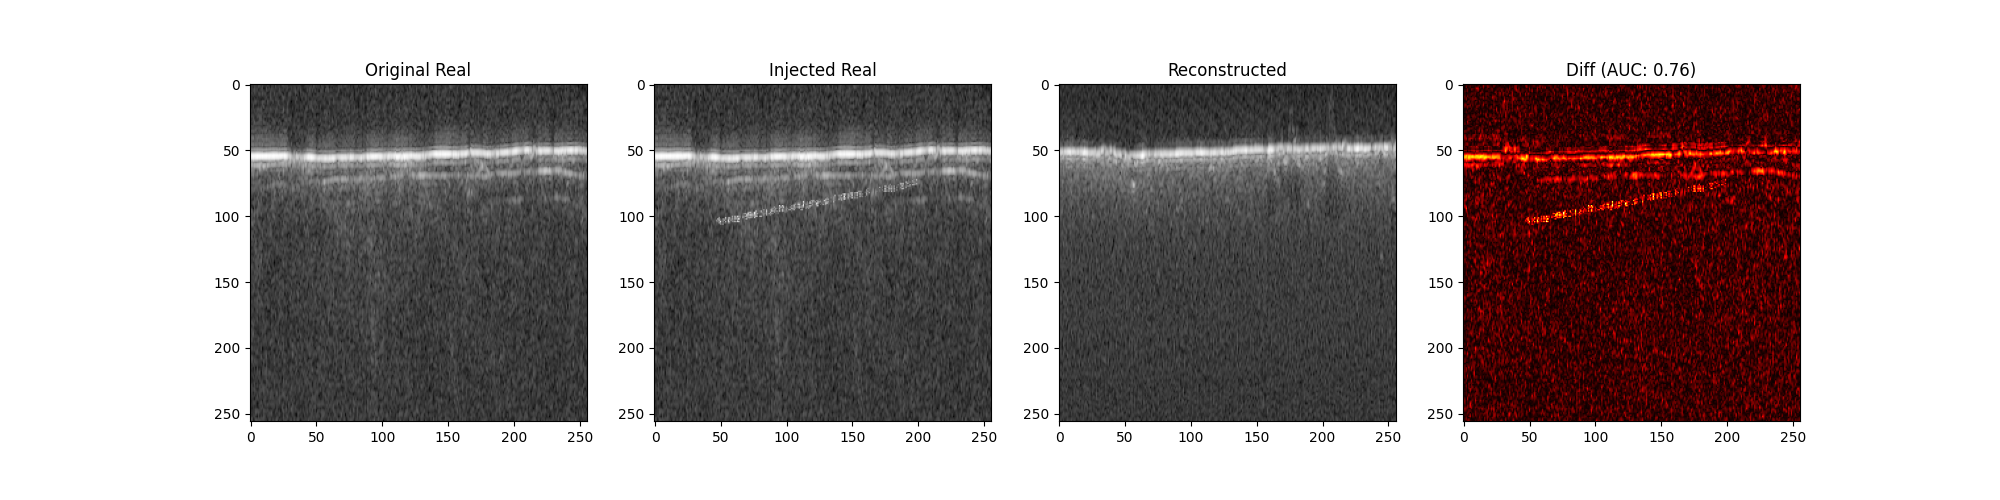
\includegraphics[width=\textwidth]{images/anomaly_eval/sample_42_auc_0.76.png}
    \caption{Example of anomaly detection on a synthetic dipping-layer injection. From left to right: (a) original real radargram, (b) radargram with synthetic injected layer, (c) CycleGAN reconstruction (background-only estimate), (d) residual map. The difference image successfully isolates the injected feature as a high-energy structure, despite the presence of strong speckle and surface clutter.}
    \label{fig:synthetic_anomaly_example}
\end{figure}

\subsection{Metric Selection and Aggregation Strategies}
\label{subsec:metric_selection}
To quantitatively evaluate the effectiveness of the different approaches, the performance of L1, L2, SSIM-based metrics, as well as \texttt{pixel-level}, \texttt{patch-based}, and \texttt{sliding-window} calculation methods were compared.

\subsubsection{Comparison of Difference Metrics}
Figure~\ref{fig:metrics_comparison} shows a comparison between the difference maps generated by the different metrics on the same sample.

\begin{itemize}
    \item \textbf{L1 (Absolute Difference):} The L1 metric proves very effective in highlighting pixel-wise differences, resulting in highly detailed but also noisier anomaly maps. It is mathematically simple but prone to flagging high-frequency background clutter and GAN artifacts as false positives.
    \item \textbf{L2 (Squared Difference):} By squaring the pixel-wise errors, the L2 metric heavily penalizes large discrepancies while aggressively suppressing low-amplitude background noise. This results in a much darker, sparser anomaly map that isolates only the strongest deviations, though it risks masking subtle, low-intensity anomalies.
    \item \textbf{1 - SSIM (Structural Dissimilarity):} Since standard SSIM measures structural similarity, we utilize $1 - \text{SSIM}$ to represent the anomaly score. Being a perceptual metric, it evaluates differences in local image geometry and texture rather than absolute pixel intensity, producing broader and more structurally coherent anomaly regions.
\end{itemize}

\begin{figure}[htbp]
    \centering
    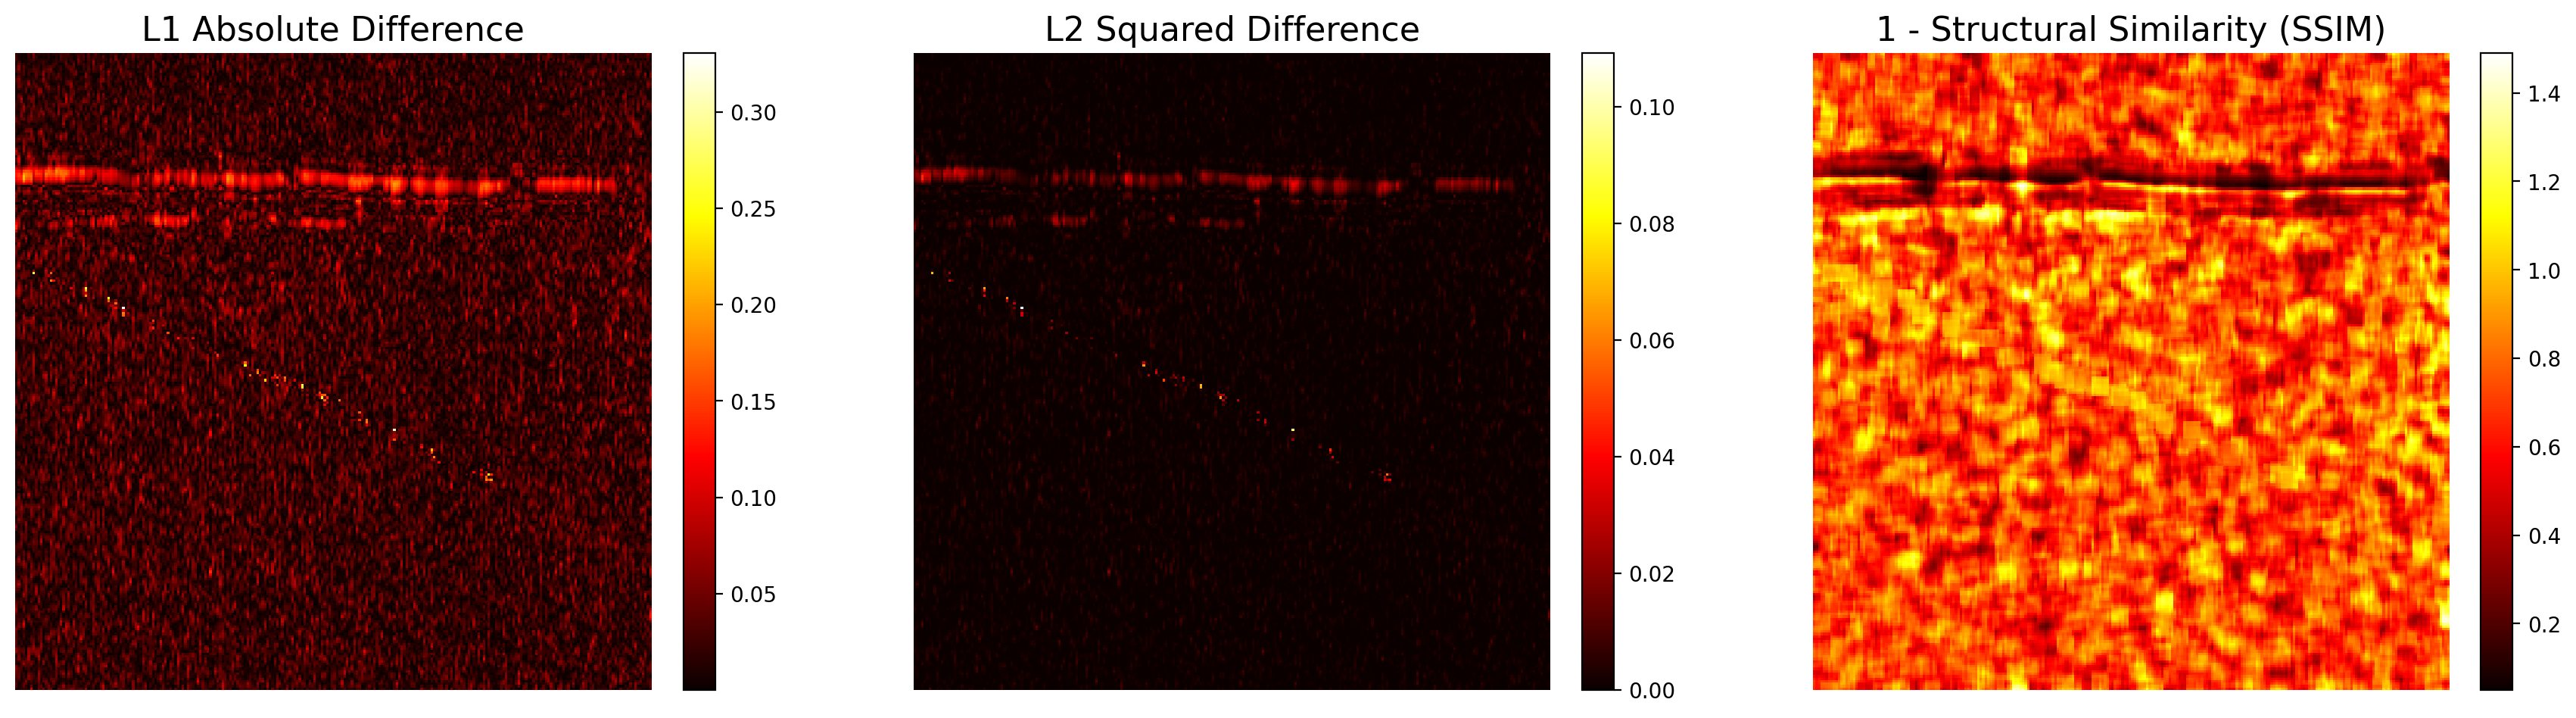
\includegraphics[width=\linewidth]{images/example_plots/thesis_plots/metric_comparison_46}
    \caption{Comparison of difference maps generated by L1, L2, and $1 - \text{SSIM}$ on the same test sample. \emph{Left:} The L1 absolute difference map highlights pixel-wise intensity discrepancies with high spatial detail but retains significant background noise. \emph{Centre:} The L2 squared difference map suppresses low-amplitude noise, isolating only the most severe intensity deviations. \emph{Right:} The $1 - \text{SSIM}$ map captures structural dissimilarities, producing smoother anomaly regions based on local texture changes.}
    \label{fig:metrics_comparison}
\end{figure}

\subsubsection{Impact of Aggregation Strategies}
The aggregation method used to compute the final anomaly score significantly impacts the robustness and interpretability of the detection map.
We evaluated three primary strategies:

\begin{itemize}
    \item \texttt{pixel-level}: While preserving maximum spatial resolution, this approach is extremely sensitive to stochastic noise and minor pixel-wise misalignments. This sensitivity frequently results in a fragmented, \enquote{salt-and-pepper} artifact pattern across the detection map, complicating the isolation of genuine anomalies.
    \item \texttt{patch-based}: By averaging error values over a fixed, non-overlapping grid (e.g., $16 \times 16$ pixels), this method reduces high-frequency noise. However, it artificially degrades the map's resolution and introduces boundary effects, risking the obfuscation of small anomalies that happen to span adjacent patches.
    \item \texttt{sliding-window}: This approach proved to be the most robust trade-off. By applying a moving average filter across the L1 difference map, it effectively smooths out high-frequency speckle noise while maintaining high spatial resolution. This method generates contiguous, well-defined anomaly regions and preserves the accurate localization of the anomaly's centroid. The progressive impact of varying the window size is illustrated in Figure~\ref{fig:sliding_window_effect}.
\end{itemize}

\begin{figure}[htbp]
    \centering
    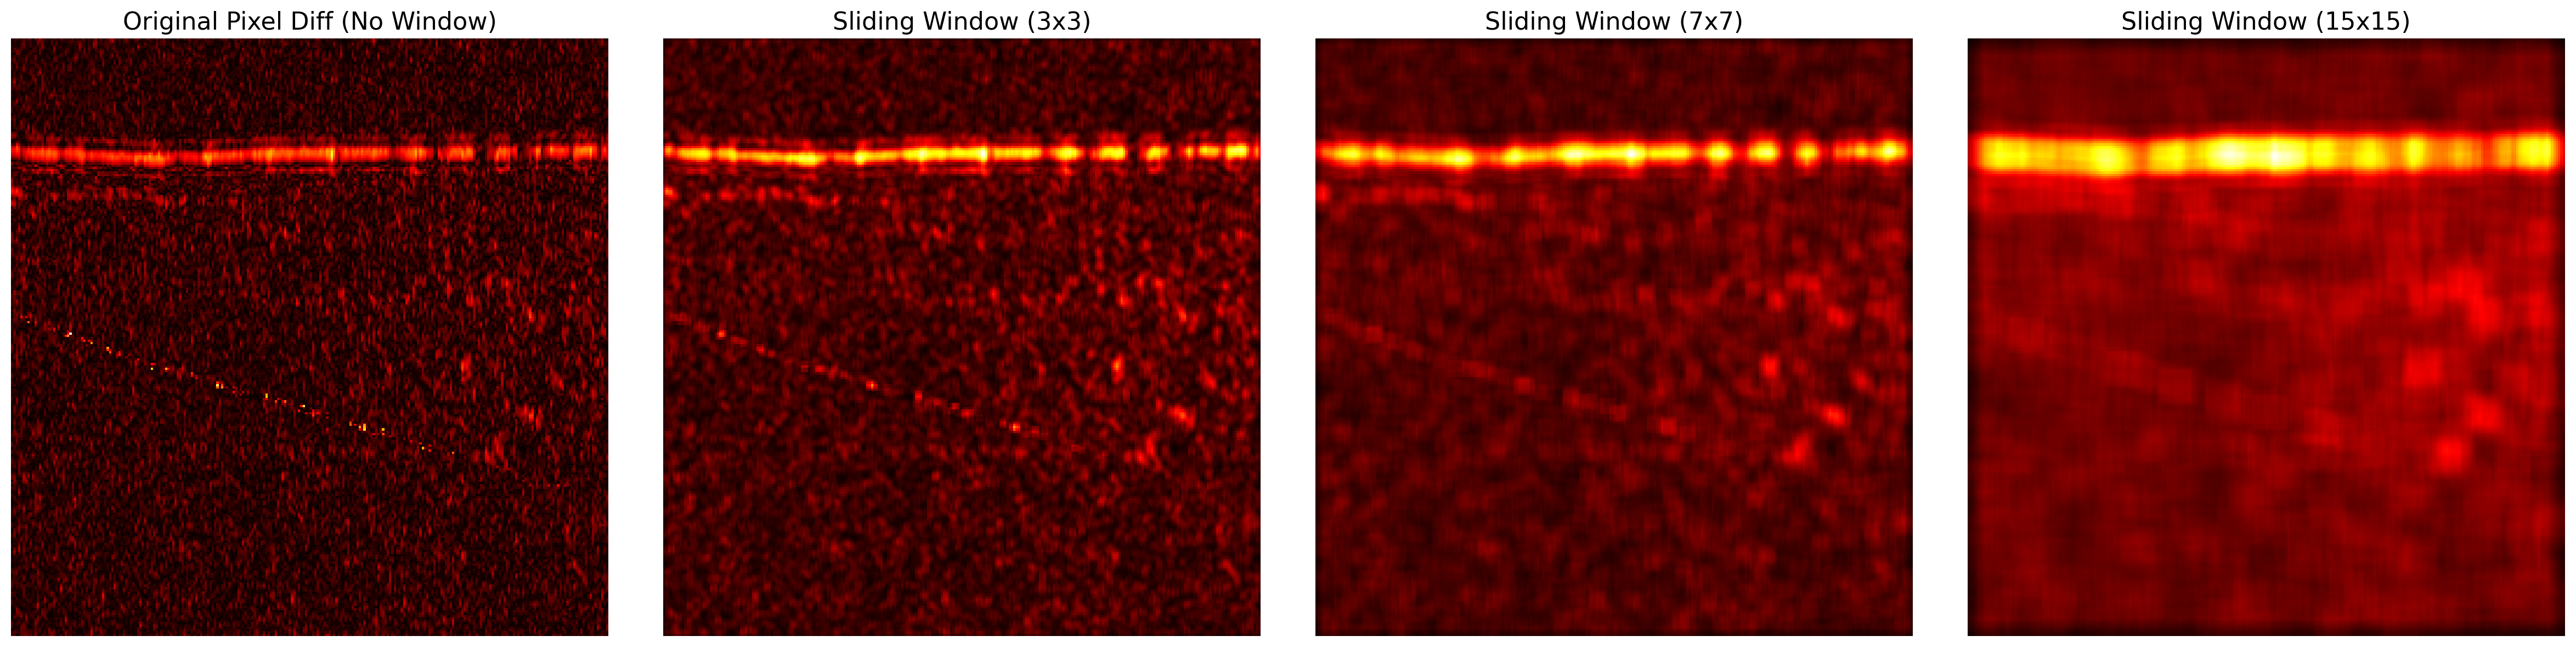
\includegraphics[width=\linewidth]{images/example_plots/thesis_plots/sliding_window_effect_59}
    \caption{Progressive effect of the \texttt{sliding-window} aggregation method on an L1 difference map. \emph{Far Left:} The original pixel-level difference map, exhibiting high detail but significant background noise. \emph{Center Left to Far Right:} The application of a moving average filter with increasing window sizes ($3\times3$, $7\times7$, and $15\times15$). As the window size increases, the high-frequency stochastic noise is effectively suppressed, consolidating the anomaly signal into a coherent, easily segmentable region, albeit with a slight loss in fine structural detail at the $15\times15$ scale.}
    \label{fig:sliding_window_effect}
\end{figure}





\subsection{Threshold Sensitivity Analysis}
\label{subsec:threshold_analysis}

The selection of the discrimination threshold $\tau$ constitutes the most critical hyperparameter in the detection subsystem, governing the trade-off between sensitivity (Recall) and false alarm rate (Precision). 
o conduct a consistent comparative study across metrics with varying native scales, the difference maps obtained from synthetic injections were locally normalized to the $[0, 1]$ range using Min-Max scaling.
We evaluated the morphological behavior of the detected anomalies at discrete threshold levels $\tau \in \{0.1, 0.3, 0.5\}$, as illustrated in Figure~\ref{fig:threshold_effect}.

We identify three main operational regimes based on the normalized threshold:
\begin{itemize}
    \item \textbf{Under-thresholding ($\tau \approx 0.1$):} The detector operates with maximum sensitivity but is overwhelmed by stochastic noise. For L1 and L2, this generates a massive amount of \textbf{false positives}, yielding a noisy detection map that requires significant manual filtering.
    \item \textbf{Optimal Balance ($\tau \approx 0.3$):} This intermediate regime represents the \enquote{sweet spot}. It effectively suppresses the majority of the background noise floor while preserving the geometric integrity and spatial compactness of the genuine subsurface anomaly.
    \item \textbf{Over-thresholding ($\tau \approx 0.5$):} Imposing a strict filter removes almost all false positives, yielding a highly precise mask. However, it risks introducing \textbf{false negatives} by fracturing the anomaly mask and erasing fainter structural details or edges that possess signal powers comparable to the residual noise floor.
\end{itemize}

\paragraph{The SSIM Inversion Phenomenon}
As visible in the bottom row of Figure~\ref{fig:threshold_effect}, the thresholded masks for the $1-\text{SSIM}$ metric appear visually inverted compared to L1 and L2 (i.e., the anomaly is black while the background is white).
This counter-intuitive behavior stems from the physical nature of synthetic radar speckle.
Since the GAN-generated high-frequency noise is spatially uncorrelated with the real background clutter, the structural dissimilarity in anomaly-free regions saturates to its maximum value ($\approx 1.0$).
Conversely, the strong, coherent reflection of the injected layer locally suppresses the variance, producing a relative drop in the dissimilarity score (creating a local minimum, $\approx 0.0$).
Consequently, applying the standard condition $M = (\mathcal{M} > \tau)$ isolates the noisy background rather than the target.
While mathematically correct within the context of structural variance, operational deployments using SSIM would require the normalized map to be inverted ($1.0 - \mathcal{M}_{norm}$) prior to thresholding to align its logic with absolute-difference metrics.

\paragraph{Low Threshold Regime ($\tau < 0.2$):}
In the low-threshold configuration, the detector operates with maximum sensitivity.
While this ensures that even faint subsurface reflections---weakened by attenuation in the crust---are captured, it introduces a substantial quantity of \textbf{false positives}.
In this regime, the system struggles to differentiate between genuine geologic features and residual GAN inaccuracies.
Specifically, slight misalignments in the phase of the generated clutter or high-frequency noise that the generator failed to perfectly replicate are flagged as anomalies.
The result is a \enquote{noisy} detection map which, while inclusive, requires significant manual filtering to identify meaningful targets.

\paragraph{High Threshold Regime ($\tau > 0.5$):}
Conversely, increasing the threshold imposes a strict filter on the residuals.
This regime effectively suppresses the stochastic noise floor and minor reconstruction errors, resulting in high Precision.
The detected regions are almost certainly strong reflectors that lack a surface correlate.
However, this rigorous filtering allows for a high rate of \textbf{false negatives}.
Weak subsurface signals, which are often the scientifically most interesting targets (e.g., deep aquifers or thin sedimentary layers), may possess signal powers comparable to the residual noise floor.
By setting $\tau$ too high, these subtle features are masked, effectively erasing the very data the system aims to uncover.

Optimal performance is typically found in an intermediate regime, often determined adaptively based on the local noise floor estimation of the current radargram.
Our experiments suggest that a static threshold is insufficient for global Mars application due to varying surface roughness and dielectric permittivity; thus, $\tau$ should be treated as a dynamic parameter adjusted per orbit.

\begin{figure}[htbp]
    \centering
    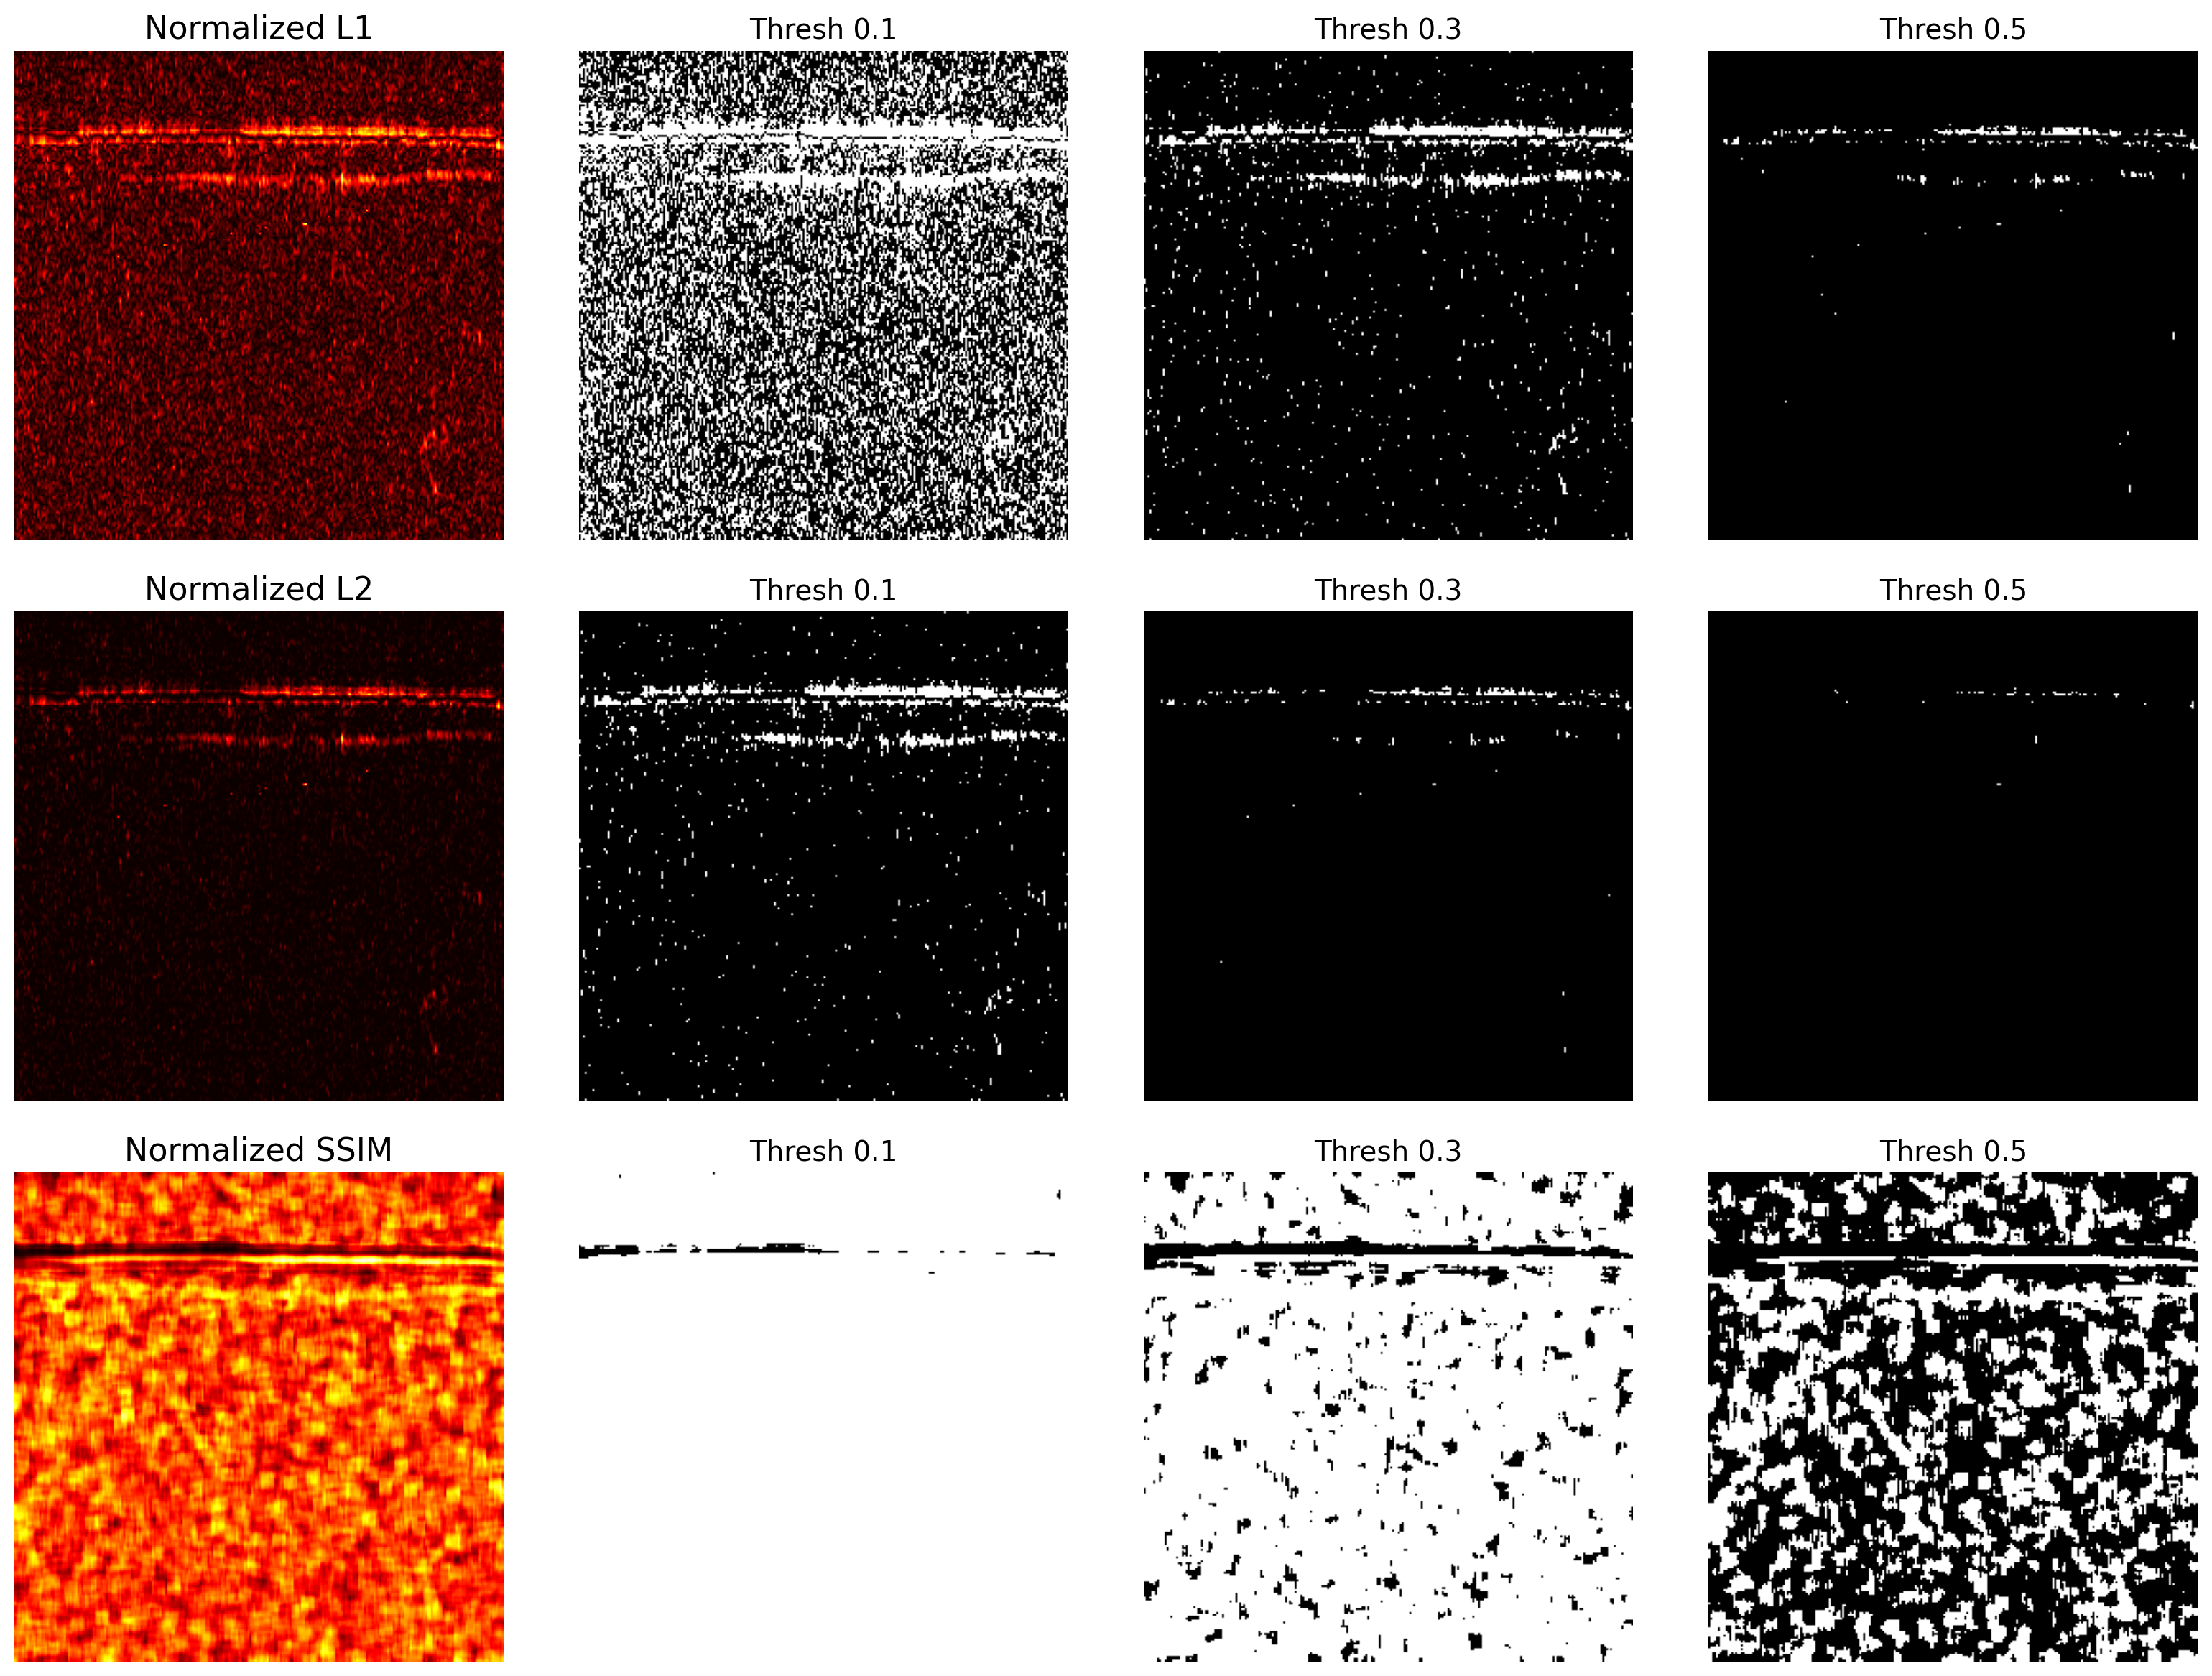
\includegraphics[width=\textwidth]{images/example_plots/thesis_plots/threshold_effect_grid_39}
    \caption{Sensitivity analysis of the discrimination threshold $\tau$ on difference maps normalized via Min-Max scaling. \emph{Top to bottom rows:} Normalized L1, L2, and $1-\text{SSIM}$ difference maps. \emph{Left to right columns:} Continuous normalized maps followed by their respective binary masks evaluated at $\tau = 0.1, 0.3,$ and $0.5$. While $\tau=0.1$ admits excessive background speckle and $\tau=0.5$ begins to erode the structural edges of the target, $\tau=0.3$ provides an optimal signal-to-noise balance for L1 and L2 metrics. The $1-\text{SSIM}$ masks exhibit an inverted logic (the target is mapped to black) due to the saturation of structural dissimilarity in the highly uncorrelated background speckle.}
    \label{fig:threshold_effect}
\end{figure}

\subsection{Operational Implications: The Human-in-the-Loop Comparison}
\label{subsec:human_in_loop}
It is imperative to contextualize these results within the broader operational workflow of planetary exploration.
The developed CycleGAN-based anomaly detector is not designed to function as a fully autonomous agent that unilaterally confirms the existence of subsurface water or structures. 

Instead, this system serves as a sophisticated \textbf{human-assistive tool}.
In the current manual workflow, researchers must painstakingly examine thousands of kilometers of SHARAD tracks, mentally filtering out complex surface reflections to spot deviations.
This process is prone to fatigue and cognitive bias.
Our model acts as an \enquote{attention mechanism,} processing terabytes of data to flag high-probability ROIs. 

By presenting the operator with the Residual Map $\mathcal{M}$ rather than the raw data alone, we reduce the cognitive load, allowing the expert to focus only on the pre-screened locations where the physics simulation and the observation diverge.
The high-recall (low threshold) configuration is therefore preferred for operational use, as it prioritizes ensuring that no potential discovery is overlooked, deferring the final validation—and the rejection of false positives—to the expert human analyst.
This \enquote{Human-in-the-Loop} architecture combines the computational throughput of Deep Learning with the geologic reasoning of a domain expert, offering a scalable path forward for the comprehensive subsurface mapping of Mars.

\subsection{Analysis of Model Behavior and Limitations in Physics Acquisition}
\label{subsec:physics_analysis}
During the testing and validation phase, a deeper analysis of the images generated by the CycleGAN model revealed an important nuance regarding the intrinsic limitation of the training process.
Although the model successfully learned to reproduce the visual appearance of real RS data, such as texture and hyperbola geometries, it remains unclear whether it genuinely internalized the physical laws governing radar signal propagation in the subsurface, or if it merely replicated the global statistical distributions of the training set.

\subsubsection{Observation of Intensity Decay}
Real RS data (radargrams) are characterized by a fundamental physical phenomenon: signal attenuation.
As electromagnetic waves penetrate the ground, their energy dissipates.
This visually translates into a decay of pixel intensity from top to bottom of the image.
The upper part of the radargram, representing the surface (or zero time), has signals with higher amplitude, while the lower part, representing greater depths, shows signals with notably reduced amplitude.

To analyze this behavior, the average normalized intensity profile was calculated for each row (depth sample) of the image, averaging over all test samples and spatial positions, for the real, simulated, and GAN-reconstructed signals.

\begin{figure}[htbp]
    \centering
    
    % --- PRIMO BLOCCO: Immagine dB ---
    \begin{subfigure}{\textwidth}
        % Minipage per l'immagine (65% della larghezza)
        \begin{minipage}[c]{0.65\textwidth}
            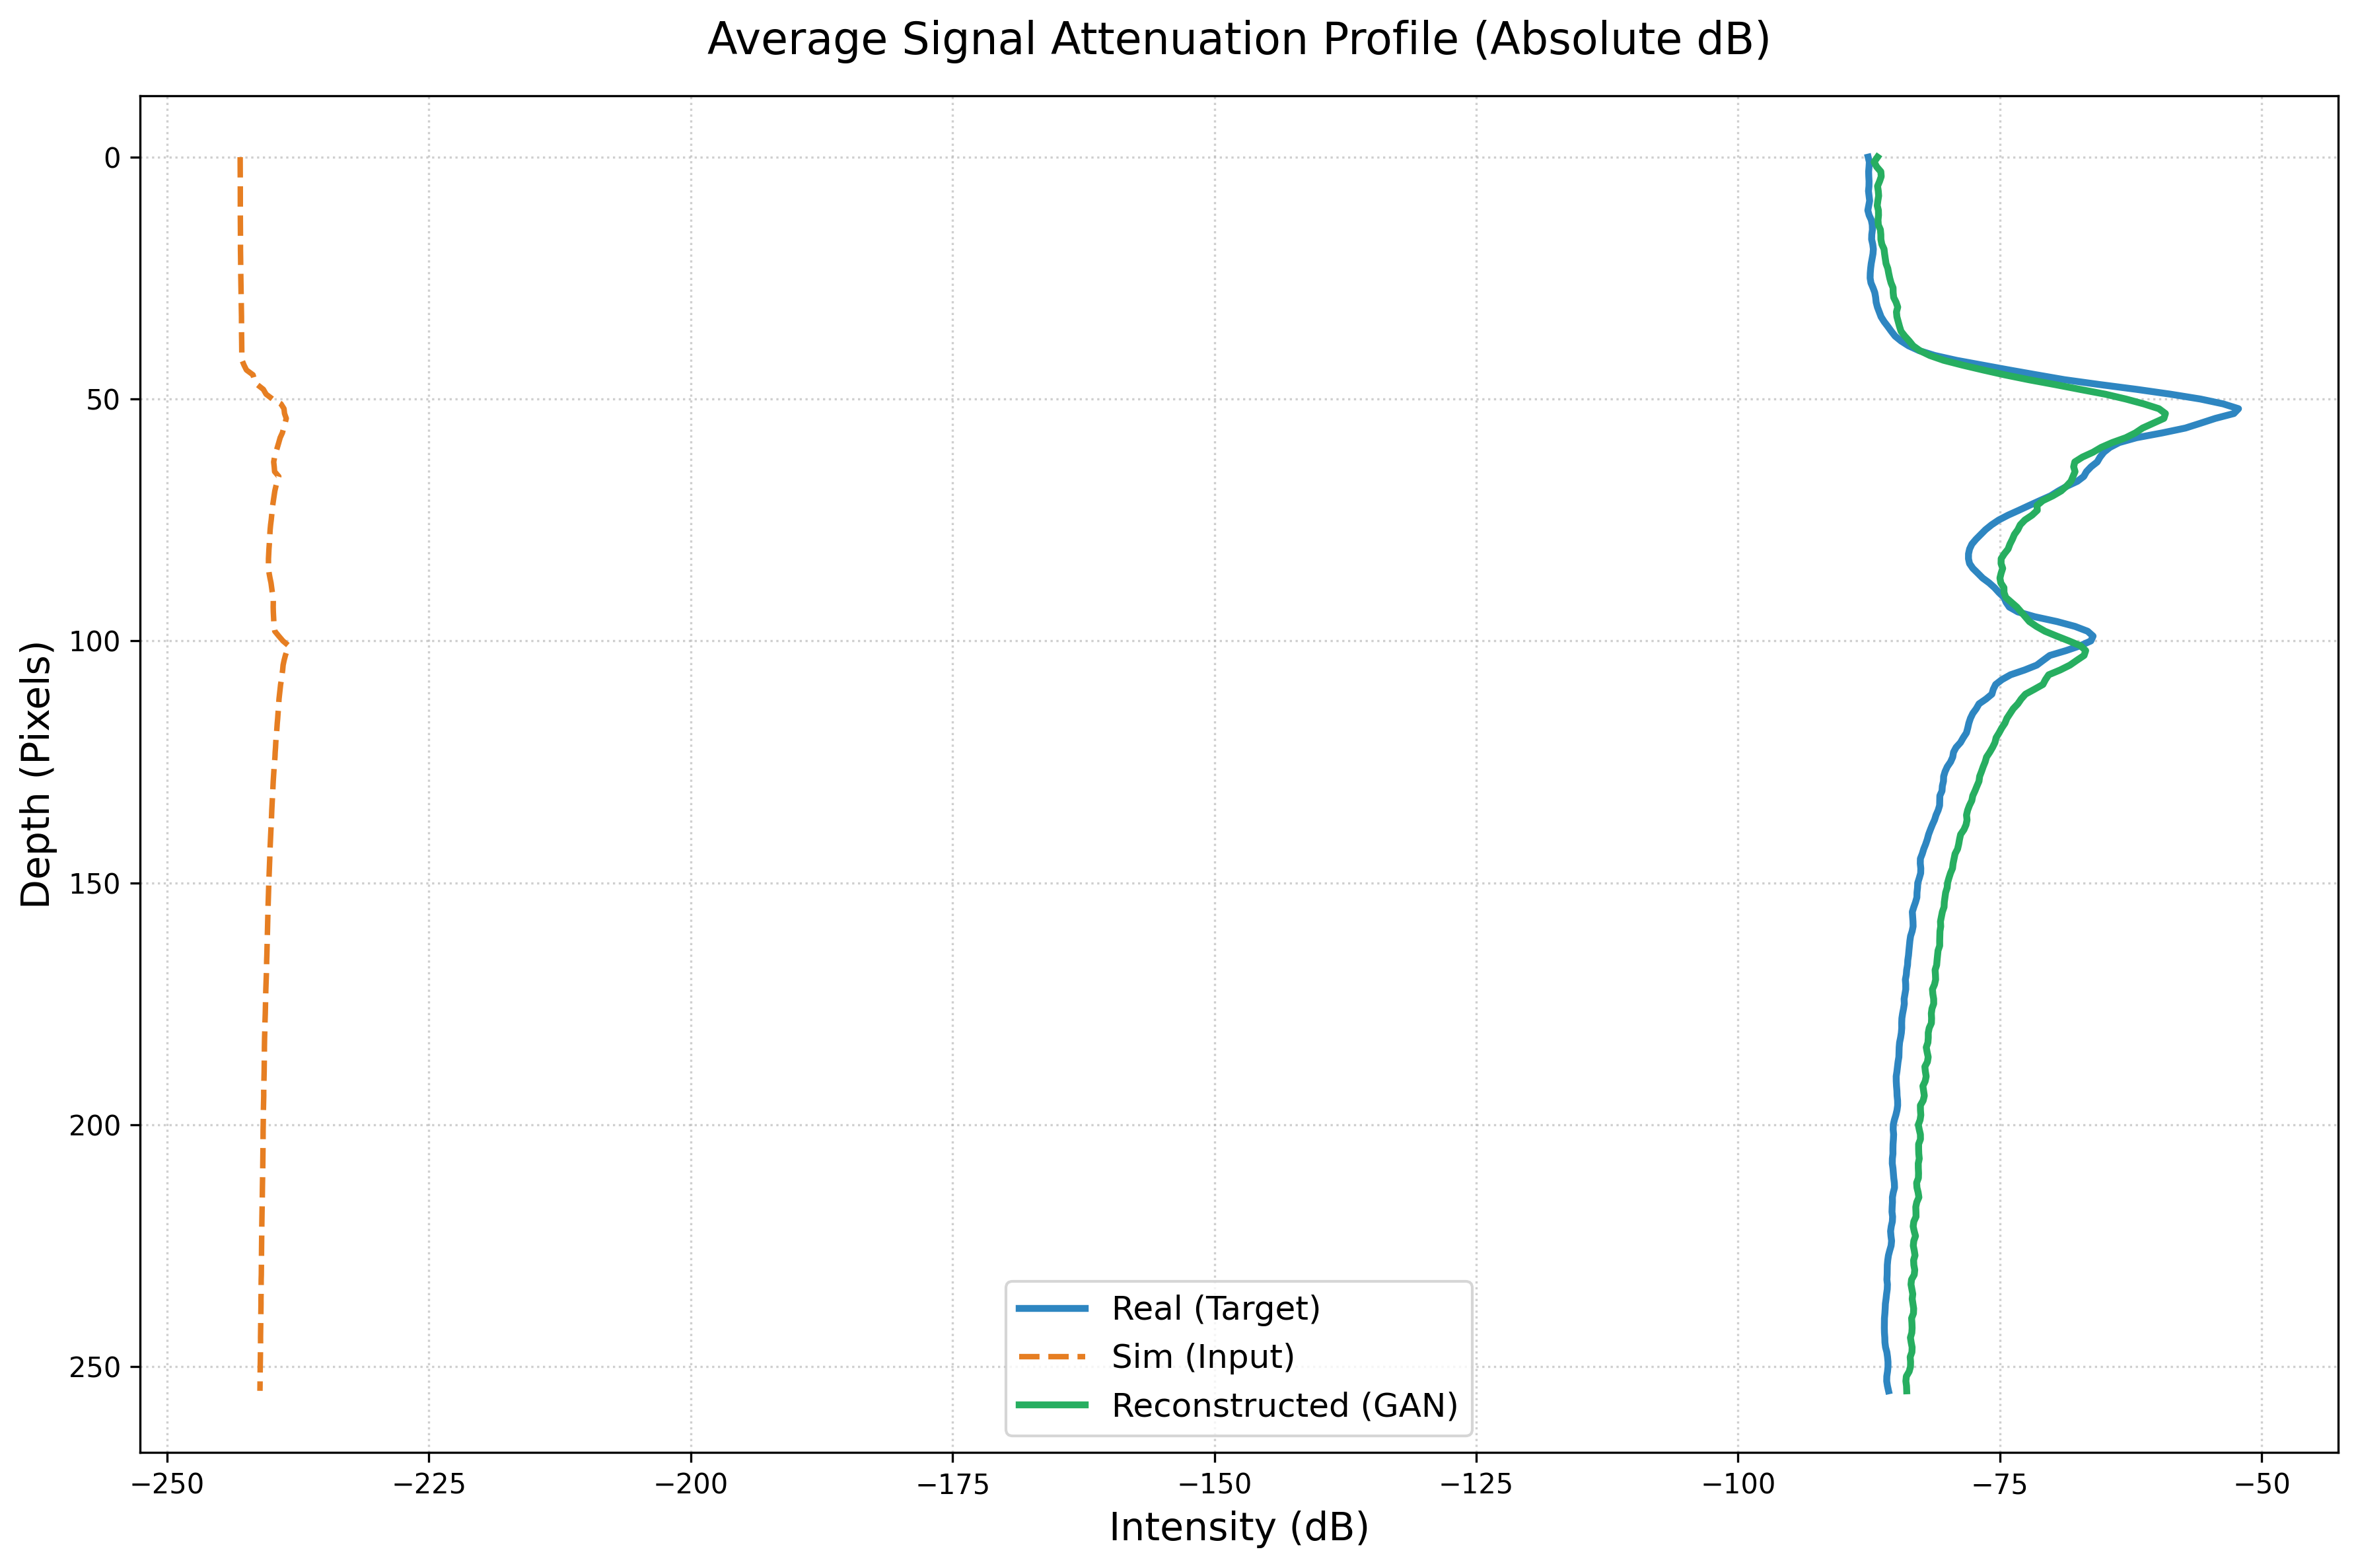
\includegraphics[width=\linewidth]{images/example_plots/thesis_plots/avg_signal_attenuation_profile_db}
        \end{minipage}\hfill
        % Minipage per la caption laterale (32% della larghezza)
        \begin{minipage}[c]{0.32\textwidth}
            \caption{Absolute intensity scale (dB). The simulation domain (dashed orange) is confined to the range $[-240, -200]$~dB, approximately $175$~dB below the real signal (solid blue). This severe domain gap motivates the use of an unpaired domain-translation approach rather than direct sim-to-real subtraction.}
            \label{fig:intensity_decay_db}
        \end{minipage}
    \end{subfigure}
    
    \vspace{0.5cm} % Spazio verticale tra i due grafici
    
    % --- SECONDO BLOCCO: Immagine Normalizzata ---
    \begin{subfigure}{\textwidth}
        % Minipage per l'immagine (65% della larghezza)
        \begin{minipage}[c]{0.65\textwidth}
            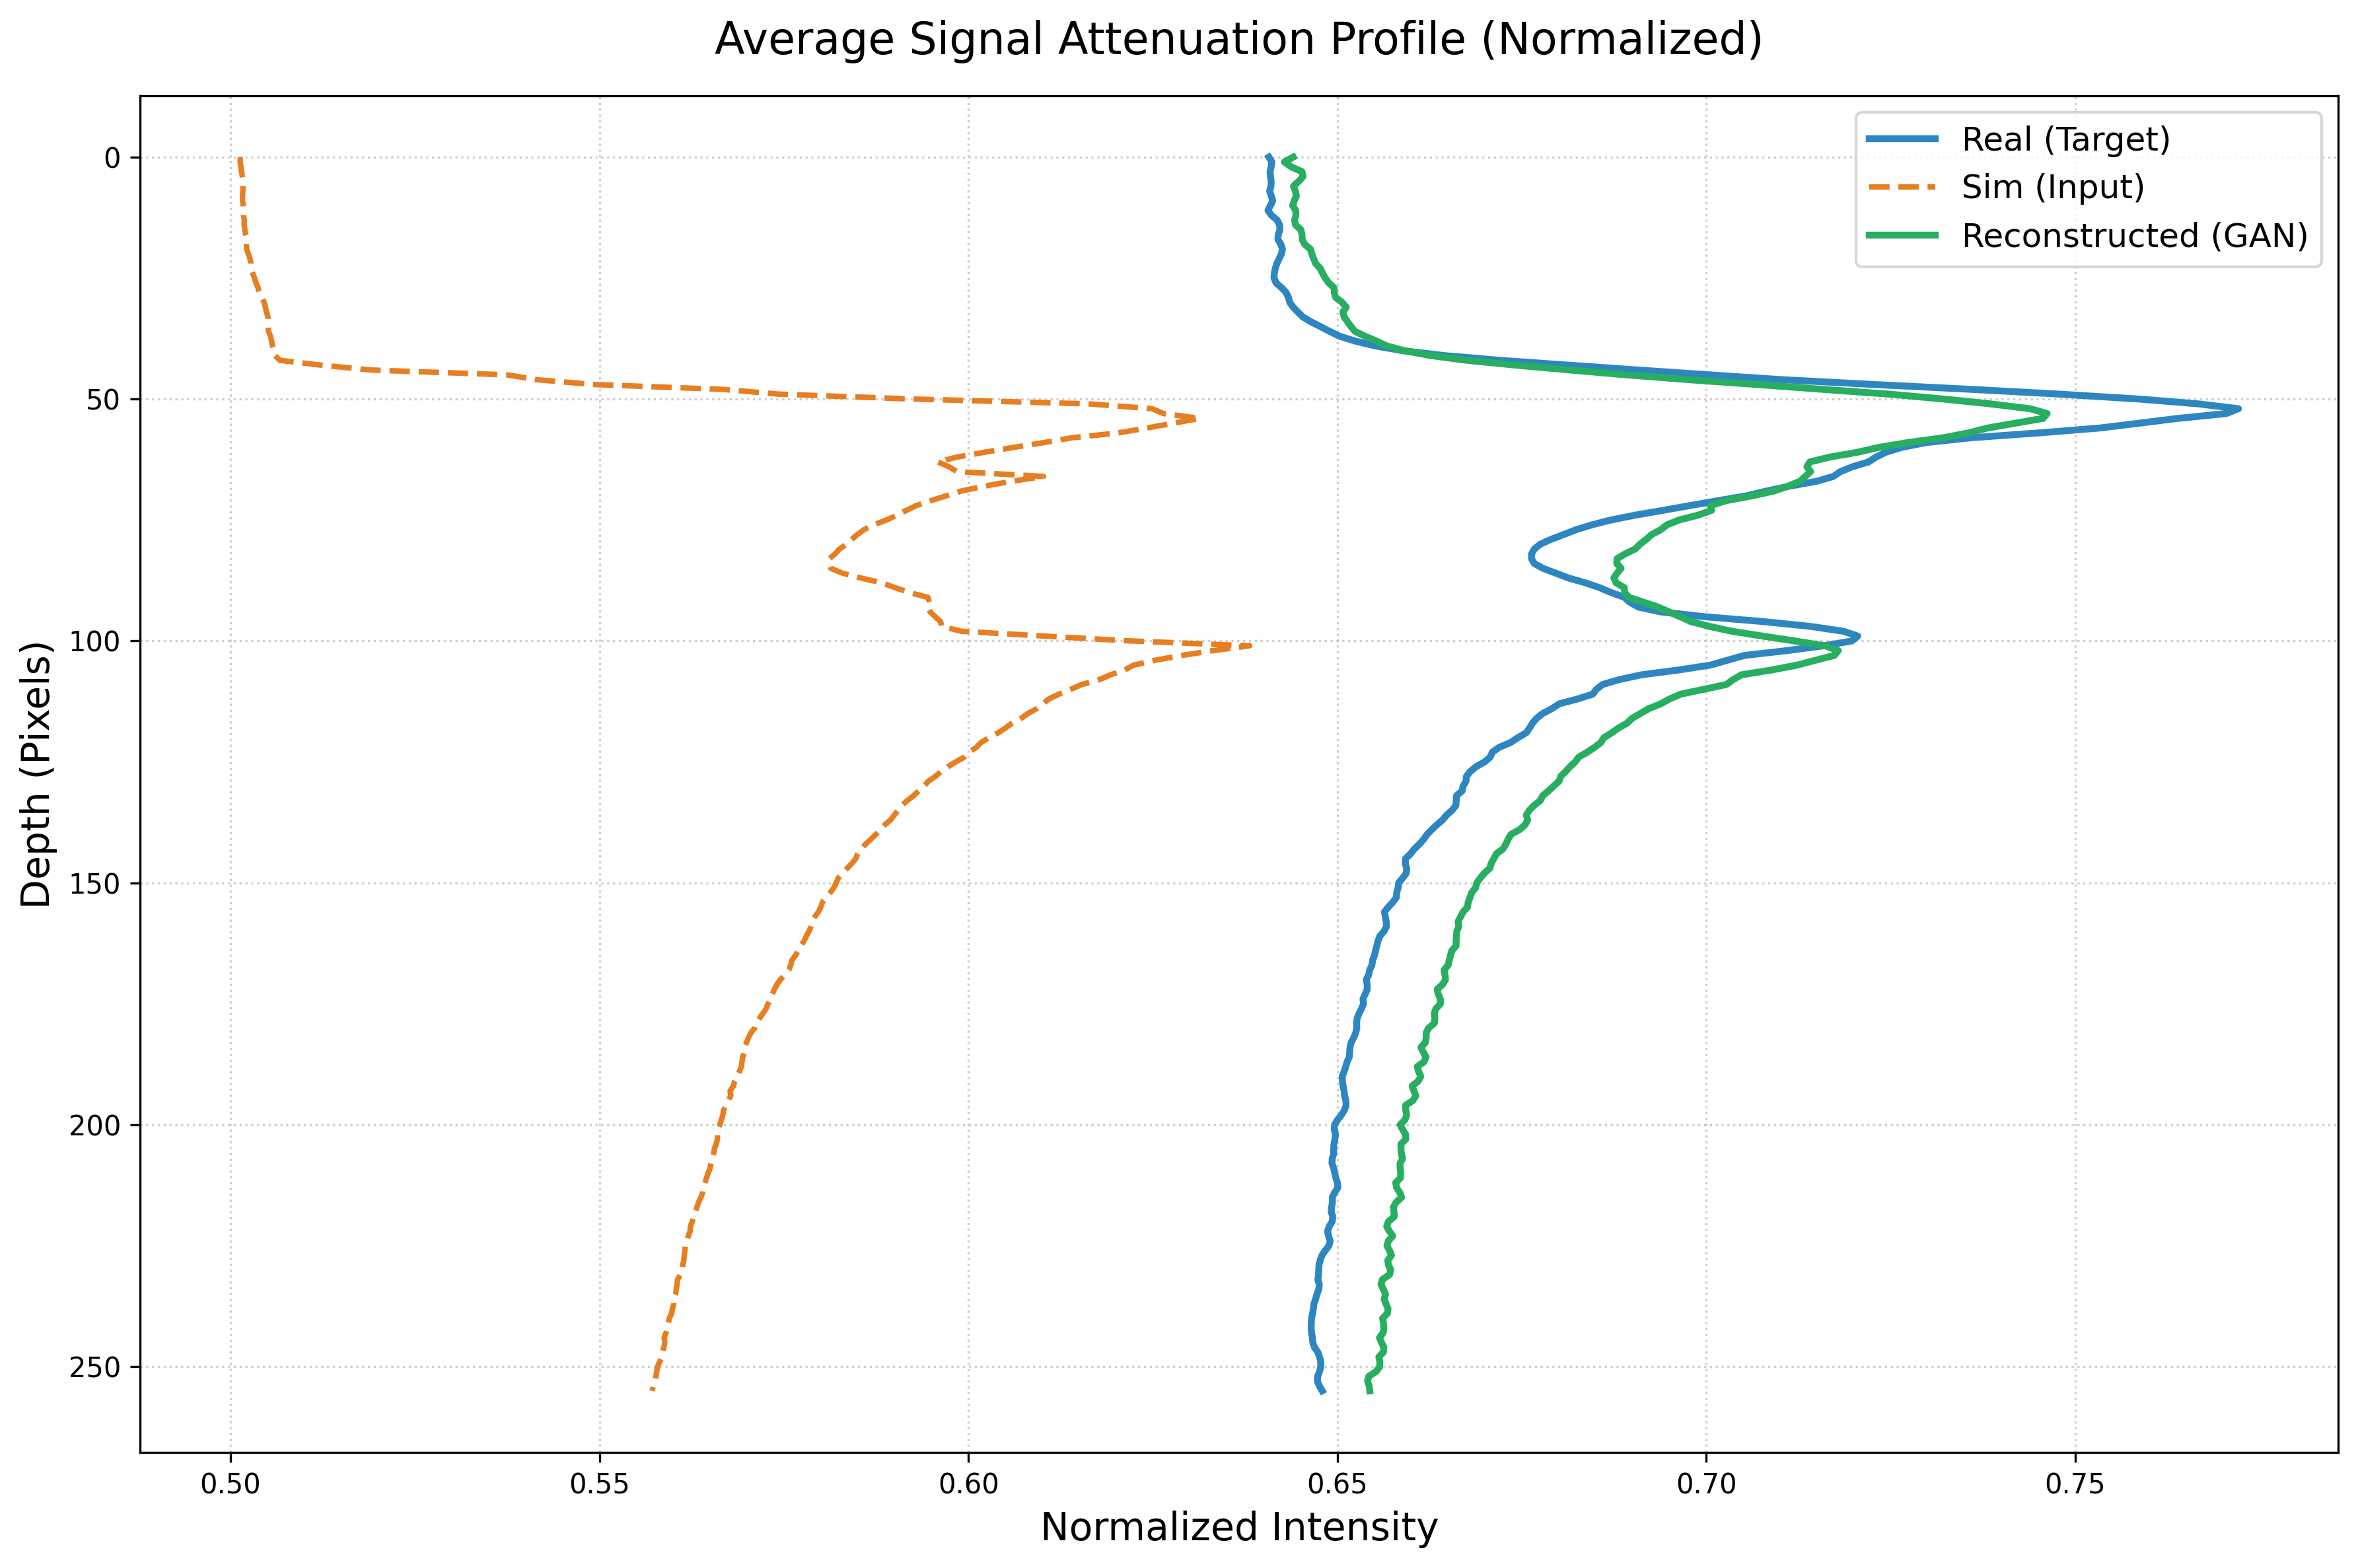
\includegraphics[width=\linewidth]{images/example_plots/thesis_plots/avg_signal_attenuation_profile_normalized}
        \end{minipage}\hfill
        % Minipage per la caption laterale (32% della larghezza)
        \begin{minipage}[c]{0.32\textwidth}
            \caption{Normalized intensity scale $[0,1]$. In this space, the CycleGAN reconstruction (solid green) closely follows the real signal profile across the depth range, suggesting that the adversarial training may have partially captured the depth-dependent energy decay from the dataset's global statistics.}
            \label{fig:intensity_decay_norm}
        \end{minipage}
    \end{subfigure}
    
    % --- CAPTION PRINCIPALE SOTTO TUTTO ---
    \caption{Average signal attenuation profiles as a function of depth for real radargrams, geometric-optics simulations, and CycleGAN reconstructions. Stacking the absolute and normalized views clarifies both the necessity of the GAN-based domain adaptation and its resulting depth-dependent behaviour.}
    \label{fig:intensity_decay}
\end{figure}

As illustrated in Figure \ref{fig:intensity_decay}, the profiles reveal three distinct behaviors:
\begin{itemize}
    \item \textbf{Real Radargrams:} Occupy the high-intensity range (${\sim}0.64$--$0.78$ normalized), exhibiting a structured depth profile with a prominent surface-echo peak near the surface and a gradual energy decrease at greater depths, consistent with electromagnetic attenuation in the Martian crust.
    \item \textbf{Simulated Radargrams:} Confined to a markedly lower normalized range (${\sim}0.50$--$0.62$), approximately $0.12$--$0.15$ normalized units below the real domain. The geometric-optics forward model captures only surface-reflected energy and entirely omits subsurface propagation losses, placing the simulation in a fundamentally different energy regime.
    \item \textbf{CycleGAN Reconstructions:} Closely follow the real signal profile across the observed depth range, suggesting that the adversarial training may have partially captured the depth-dependent energy decay. This behaviour is encouraging, but should be interpreted with caution: the PatchGAN discriminator operates on local image patches and has no explicit access to global depth statistics, so the apparent attenuation trend may reflect a statistical regularity of the training distribution rather than a genuine internalization of the underlying electromagnetic physics. Dedicated experiments (such as evaluating the model on patches extracted from different orbital tracks, varying surface conditions, or artificially modified attenuation profiles) would be needed to distinguish between these two hypotheses.
\end{itemize}

A complementary analysis of per-column intensity histograms (A-scans) shows that the distributions of real and reconstructed signals are broadly consistent across depth levels, without the pronounced systematic offset that would be expected from a completely physics-unaware model.
While this is consistent with the hypothesis of partial attenuation learning, it does not constitute conclusive evidence: a model that simply reproduces the marginal intensity statistics of the training set would produce similar histograms without having internalized any causal physical mechanism.

\subsubsection{Discussion: Style Learning vs.\ Physics Acquisition}
We believe the observed depth-dependent intensity profile of the reconstruction is most plausibly explained by the statistical structure of the training data rather than by genuine physics acquisition, for reasons rooted in the nature of the CycleGAN objective functions.

\begin{itemize}
    \item \textbf{Focus on Style and Texture:} The primary objective of CycleGAN is style translation between two image domains. The \textit{adversarial loss}, particularly with a PatchGAN discriminator, pushes the generator to create image patches (e.g., 70x70 pixels) that are indistinguishable from those of the target domain. This mechanism is extremely effective in learning local characteristics like soil grain texture or hyperbola shapes, but struggles to capture global image properties, such as a large-scale intensity gradient. The model found a strategy to satisfy the discriminator: it learned to reproduce not only the local texture statistics of the real domain, and may have captured global energy trends such as depth-dependent attenuation. However, since the PatchGAN discriminator evaluates local patches independently, it provides no direct supervision over global depth profiles; any apparent attenuation in the output is therefore more likely a by-product of the training data distribution than an explicitly acquired physical law.

    \item \textbf{Absence of Physical Constraints in Losses:} Standard CycleGAN cost functions (\textit{adversarial loss}, \textit{cycle consistency loss}, and \textit{identity loss}) do not contain any term enforcing adherence to physical laws. The \textit{cycle consistency loss} ($||G_{BA}(G_{AB}(A)) - A||_1$) ensures that an image can be translated and returned to its original state, but does not guarantee that the intermediate translation ($G_{AB}(A)$) is physically plausible.
\end{itemize}

This is a well-known limitation of standard GANs when applied to scientific problems.
Research in this field is moving towards so-called \textbf{Physics-Informed Neural Networks (PINNs)} and \textbf{Physics-Informed GANs}, which integrate partial differential equations (PDEs) or other physical constraints directly into cost functions to guide training towards physically coherent solutions \cite{raissi2019physics}.

\subsubsection{Impact on Anomaly Detection Results}

This discrepancy between the real and reconstructed domain has a direct impact on the anomaly detection pipeline, which relies on the comparison between the real image and its \enquote{healthy} (anomaly-free) reconstruction.

\begin{itemize}
    \item \textbf{Residual Bias in Difference Maps:} The attenuation profile analysis suggests that the GAN reconstruction does not introduce a strong systematic depth-dependent bias in the difference maps, which is an encouraging finding for the anomaly detection pipeline. Nevertheless, it remains unclear whether the model has genuinely internalized the physics of attenuation or merely replicated a statistical trend. Residual intensity mismatches cannot therefore be excluded, particularly in deeper zones or under surface conditions that are not well represented in the training set. These mismatches can produce spurious high-energy regions in the residual maps, leading to localized \textbf{false positives} whose depth distribution may vary with acquisition geometry and surface roughness.
    \item \textbf{Need for Additional Normalization:} To mitigate, at least partially, the intensity bias problem, it became necessary to introduce an additional normalization step exclusively in the anomaly detection pipeline. As described in the action plan, the introduction of \textbf{Z-score normalization} for L1/L2 metrics, applied independently to the real and reconstructed image before difference calculation, allows comparing the two images based on their relative structural variations rather than their absolute intensity values.
    
    Z-score normalization transforms each image to have mean 0 and standard deviation 1:
    \begin{equation}
        I_{norm} = \frac{I - \mu(I)}{\sigma(I) + \epsilon}
    \end{equation}
    This step mitigates residual intensity mismatches between real and reconstructed signals regardless of their origin, whether due to incomplete physics acquisition or domain shift, producing more reliable anomaly maps and reducing depth-dependent false positives.
\end{itemize}

In conclusion, the analysis reveals that the CycleGAN reconstruction closely follows the depth-dependent intensity profile of real radargrams, which is consistent with a partial internalization of signal attenuation.
However, the standard CycleGAN objective provides no explicit physical supervision, and the observed behaviour is equally consistent with a model that has learned a statistical regularity of the training distribution without internalizing the underlying electromagnetic laws.
Distinguishing between these two interpretations requires dedicated experiments.
Examples include evaluating the model on radargrams with atypical attenuation profiles, varying the geographic region, or probing the response to out-of-distribution depth patterns.
This constitutes an important direction for future work.


